%; whizzy paragraph
%; whizzy-paragraph "^\\\\dancersection"
% -initex iniptex -latex platex -format platex -bibtex jbibtex -fmt fmt
% 以上 whizzytex を使用する場合の設定。

%     Tokyo Debian Meeting resources
%     Kansai Debian Meeting resources
%     Copyright (C) 2012 Junichi Uekawa
%     Copyright (C) 2012 Nobuhiro Iwamatsu
%     Copyright (C) 2012 Koichi Akabe

%     This program is free software; you can redistribute it and/or modify
%     it under the terms of the GNU General Public License as published by
%     the Free Software Foundation; either version 2 of the License, or
%     (at your option) any later version.

%     This program is distributed in the hope that it will be useful,
%     but WITHOUT ANY WARRANTY; without even the implied warranty of
%     MERCHANTABILITY or FITNESS FOR A PARTICULAR PURPOSE.  See the
%     GNU General Public License for more details.

%     You should have received a copy of the GNU General Public License
%     along with this program; if not, write to the Free Software
%     Foundation, Inc., 51 Franklin St, Fifth Floor, Boston, MA  02110-1301 USA

%  preview (shell-command (concat "evince " (replace-regexp-in-string "tex$" "pdf"(buffer-file-name)) "&"))
% 画像ファイルを処理するためにはebbを利用してboundingboxを作成。
%(shell-command "cd image2012-natsu; ebb *.png")

% progress memo:
% 2018/12-2019/05東京がマージ対象
% 2019/07リリースパーティネタも可能なら収録
% イベント等でない場合は理由を書くこと。
% 必要な変更点は FIXME で記録しています。

%%ここからヘッダ開始。

\documentclass[mingoth,a4paper]{jsarticle}
\usepackage{monthlyreport}
\usepackage{supertabular}
\usepackage{subfigure}
\renewcommand*\thesubfigure{}

\usepackage{comment}

% section の代わりの環境 -- 改訂する。
\renewcommand{\dancersection}[2]{%
\newpage
あんどきゅめんてっど でびあん 2019年夏号
%
% top line
\vspace{0.1mm}\\
{\color{dancerdarkblue}\rule{\hsize}{2mm}}

%
% middle text
%
\begin{minipage}[t]{0.6\hsize}
\color{dancerdarkblue}
\vspace{1cm}
\section{#1}
\hfill{}#2\\
\end{minipage}
\begin{minipage}[t]{0.4\hsize}
\vspace{-2cm}
\hfill{}
\includegraphics[height=8cm]{image200502/openlogo-nd.eps}\\
\vspace{-5cm}
\end{minipage}
%
% bottom line
{\color{dancerlightblue}\rule{0.66\hsize}{2mm}}
%
\vspace{2cm}
}
% end of dancersection.

\begin{document}

\begin{titlepage}
\thispagestyle{empty}

\hspace*{-2.5cm}
\includegraphics{image2012-natsu/gudeb.eps}\\
\vspace*{0.1cm}

\vspace*{2cm}
\rotatebox{10}{\fontsize{32}{32} {\gt 東京エリア/関西Debian勉強会}}

\vspace*{-1.5cm}
\hspace*{11cm}
\includegraphics[height=6cm]{image200502/openlogo-nd.eps}\\
\vspace*{0.1cm}
\hfill あんどきゅめんてっど でびあん 2019年夏号 2019年8月12日 初版発行
\end{titlepage}

\newpage
\thispagestyle{empty}\mbox{}
\newpage

\setcounter{page}{1}
\begin{minipage}[]{0.2\hsize}
 \definecolor{titleback}{gray}{0.9}
 \colorbox{dancerlightblue}{\rotatebox{90}{\fontsize{80}{80}
{\gt \color{dancerdarkblue}デビアン勉強会} }}
\end{minipage}
\begin{minipage}[]{0.8\hsize}
\hrule
\vspace{1mm}
\hrule
\setcounter{tocdepth}{1}
{\small
\begin{multicols}{2}
  \tableofcontents
\end{multicols}
} %FIXME: does not fit in one column! しかし二段にするとあまり美しくない? 真ん中のあたりで章番号とページ数の番号が近くにあるのがバランス良くない気がする
\vspace{1mm}
\hrule
\vspace{3cm}

\end{minipage}

% FIXME: 本文を追加すること。
%-------------------------------------------------------------------------------
\dancersection{Introduction}{ }
%-------------------------------------------------------------------------------

\subsection{東京エリアDebian勉強会}

 Debian勉強会へようこそ。これからDebianの世界にあしを踏み入れると
 いう方も、すでにどっぷりとつかっているという方も、月に一回Debianについ
 て語りませんか?

 Debian勉強会の目的は下記です。

\begin{itemize}
 \item \underline{Debian Developer} (開発者)の育成。
 \item 日本語での「\underline{開発に関する情報}」を整理してまとめ、アップデートする。
 \item \underline{場}の提供。
 \begin{itemize}
  \item 普段ばらばらな場所にいる人々が face-to-face で出会える場を提供
	する。
  \item Debian のためになることを語る場を提供する。
  \item Debianについて語る場を提供する。
 \end{itemize}
\end{itemize}

 Debianの勉強会ということで究極的には参加者全員がDebian Packageをがりがり
 と作るスーパーハッカーになった姿を妄想しています。情報の共有・活用を通し
 て Debianの今後の能動的な展開への土台として、「場」としての空間を提供す
 るのが目的です。

\subsection{関西 Debian 勉強会}

 関西 Debian 勉強会はDebian GNU/Linux のさまざ
 まなトピック(新しいパッケージ、Debian 特有の機能の仕組、Debian 界隈で起
 こった出来事、などなど)について話し合う会です。

 目的として次の三つを考えています。
 \begin{itemize}
  \item メーリングリストや掲示板ではなく、直接顔を合わせる事での情報交換の促進
  \item 定期的に集まれる場所
  \item 資料の作成
 \end{itemize}

 それでは、楽しい一時をお楽しみ下さい。

%201902
%-------------------------------------------------------------------------------
\dancersection{Debian Update}{杉本}
%-------------------------------------------------------------------------------
\subsection{目次}

  \begin{itemize}
  \item Debian とは?
  \item Debian JP Project と Debian 勉強会
  \item Debian 10 (Buster)
  \item Debian Updates
  \item 今後のイベント
  \end{itemize}


%-------------------

\subsection{Debian とは?}

{\color{red}{フリー/オープン}}な{\color{red}{ユニバーサル}}オペレーティングシステム を作成しようとするボランティアベースのプロジェクト

\begin{table}[htb]
  \begin{center}
  \begin{tabular}{|c|c|c|}
    \hline
    ディストリ & 企業 & ボランティア \\ \hline
    Fedora & RedHat支援あり & あり  \\ \hline
    RHEL & RedHat & なし  \\ \hline
    CentOS & RedHat支援あり & あり \\ \hline
    \color{red}{Debian}  & \color{red}{なし} & \color{red}{あり} \\ \hline
    Ubuntu  & Canonical & あり \\ \hline
    openSUSE & SUSE支援あり & あり \\ \hline
    SLES & SUSE & なし \\ \hline
  \end{tabular}
  \end{center}
\end{table}



 世界規模で開発が行われており、63ヶ国、約1000名のDebian公式開発者が開発を行
 っている。パッケージメンテナや翻訳などの貢献者も入れるともっと多くの開発者が参加
 していることになる。
 \begin{center}
%%%   \includegraphics[width=0.7\hsize]{image201707/group_photo_t.jpg}
 \end{center}

\begin{itemize}
  \item 様々な用途に使える汎用的な作り
    \begin{itemize}
    \item デスクトップPC、ノートPCなどの普段利用するコンピュータのOS
    \item Linuxサーバ (例:webサーバのシェア:\url{https://w3techs.com/technologies/details/os-linux/all/all})
    \item 組込デバイスのベースOS (多くのCPUで動作する)
  \end{itemize}
  \item 「Debian」ベースな派生OSの源流
  \begin{itemize}
    \item Ubuntu や Raspbian といったディストリビューションのベースはDebian
    \item 派生先のディストリビューションと相互に情報交換をして開発している
  \end{itemize}
\end{itemize}




\begin{itemize}
  \item 2019年2月の時点で、最新版は {\color{red}{Debian 9.8}} (コードネーム: Stretch)
  \begin{itemize}
    \item パッケージ数は{\color{red}{約51000}}を提供
    \item 公式にサポートするCPUアーキテクチャは{\color{red}{10}}
  \end{itemize}
  \item {\color{red}{約2年毎}}にリリース
  \item 次のリリース Debian 10 (コードネーム: {\color{red}{}}Buster)は 2019年中頃にリリースすると思われる
  \item コードネームはトイ・ストーリーのキャラクターを採用
\end{itemize}




\begin{itemize}
  \item Debian 社会契約
    \begin{itemize}
      \item Debian 開発者たちが目指すフリーソフトウェアコミュニティーの在り方
    \end{itemize}
  \item Debian フリーソフトウェアガイドライン(DFSG)
    \begin{itemize}
      \item Debian 社会契約の一部
      \item Debian が考えるフリーソフトウェアの定義
      \item オープンソースの定義のひな形にもなっている
    \end{itemize}
  \item Debian Policy
    \begin{itemize}
      \item \url{https://www.debian.org/doc/debian-policy/}
      \item Debian パッケージの区分、内容やルール、ファイル配置の方針を定義
    \end{itemize}
\end{itemize}




まとめると
\begin{itemize}
  \item Debianはフリー/オープンなオペレーティングシステム (OS)を作成しようとするボランティアベースのプロジェクト
  \item 自分たちの考えるフリーという言葉に関する定義、開発目的、パッケージングポリシーを厳格に決めている
  \item 世界中に1000人以上の開発者がおり、他のディストリビューションのベースとして採用されている
  \item 約2年毎にリリースが行われ、多くのパッケージとアーキテクチャをサポートしている
  \item 上記のような特徴から様々なところで利用されているLinuxディストリビューション
\end{itemize}



%------------------


\subsection{Debian JP Projectとは}
  
\begin{itemize}
  \item 日本でDebianを普及させることを目的とした任意団体
  \item 活動内容
  \begin{itemize}
    \item Debian の日本語による情報発信
    \item ユーザとの情報交換
    \item Debian 開発者、パッケージメンテナの育成など
  \end{itemize}
\end{itemize}



\subsection{Debian勉強会}
  
\begin{itemize}
 \item 2005年1月開始
 \item Debian Developer 上川さん発起人
\item 東京と関西で月に一回コンスタントに開催しているDebian開発者、ユーザによる勉強会
\end{itemize}





\subsection{Debian勉強会:解決したい内容}
\begin{itemize}
 \item 問題
    \begin{itemize}
	\item MLとIRCで情報交換していた
	\item face-to-faceであう場所がない
	\item まとまったドキュメントが出てこない
    \end{itemize}
 \item Debian勉強会の提案
    \begin{itemize}
	\item 定期的に集まる
	\item 資料を作成する。(GPLで!) \\
	  {\small \url{https://salsa.debian.org/tokyodebian-team/monthly-report}}
    \end{itemize}
\end{itemize}





%-----------------------

\subsection{最新安定版 Debian 10 (Buster)}

  %\begin{center}\Huge{Debian 10 (Buster)}\end{center}
  %\begin{center}\Huge{Debian 10 (Buster)\\リリースおめでとう!}\end{center}

Debian 10 には「Buster」というコードネームをつけています。

\begin{itemize}
%\item 現在開発を進めている次の安定版リリース
\item Debianはtime-based freezeを採用しており、およそ2年毎のリリースを目指す
\end{itemize}
  \begin{center}
    %\includegraphics[width=0.6\hsize]{image201902/buster.jpg}
    % https://pixar.fandom.com/wiki/Buster
  \end{center}



\subsubsection{テーマ}



テーマはAlex Makasさん提案の「futurePrototype」に決定。
  
\begin{center}
  
\includegraphics[width=0.75\hsize]{image201902/futurePrototype-wallpaper-1920x1080_gray.png}
\end{center}

\url{https://bits.debian.org/tag/artwork.html}

\url{https://wiki.debian.org/DebianArt/Themes/futurePrototype}




\subsubsection{提供ソフトウェアのバージョン}



ソフトウェアは以下のバージョンでテスト中

\begin{itemize}
\item Linux カーネル 4.19
\item ツールチェイン(GCC 8.2.0, binutils 2.31.1, glibc 2.28), LLVM 7.0.1, 6.0.1
\item Perl 5.28.1, Python 2.7.15/3.7.2, Ruby 2.5.1, PHP 7.3.2, Go 1.11.5, OpenJDK 11.0.2, 8u171
\item GNOME 3.30, KDE 5.14.5, Cinnamon 3.8.8, MATE 1.20, Xfce 4.12.5, lxde 0.99.0, lxqt 0.14.0
\item MariaDB 10.3.12, PostgreSQL 11.1, sqlite 3.26.0, 2.8.17 
\item OpenSSH 7.9p1, OpenSSL 1.1.1a, GnuPG 2.2.12/1.4.23
\item etc..
\end{itemize}




\subsubsection{インストーラ}


Debian Installer Buster Alpha 5 Release

\begin{itemize}
  \item \url{https://www.debian.org/devel/debian-installer/News/2019/20190202}
  \item いち早くBusterを試してみたい方は以下からダウンロードしてインストールできます。
  \begin{itemize}
    \item \url{https://www.debian.org/devel/debian-installer/index.ja.html}
  \end{itemize}
\end{itemize}




\subsubsection{リリースまでの流れ}

  %\begin{center}\Huge{Debian 10 (Buster)\\Soft freeze突入}\end{center}


Debian 10のリリースまでの流れ \\
\url{https://wiki.debian.org/DebianBuster}
  
\begin{itemize}
\item 2019-01-12: Transition freeze
  \begin{itemize}
  \item これ以降、大規模な変更や他のパッケージに大きな影響を与える変更を行ってはいけない
  \end{itemize}
\item 2019-02-12: Soft freeze ←今はこの段階
  \begin{itemize}
  \item 変更は小規模で的を絞った内容に限って行う
  \item 例)バグ修正、セキュリティ修正、他のパッケージとの調整
  \item この期日までにtestingに移行していないパッケージは次のリリースに含まれません
  \end{itemize}
\item 2019-03-12: Full freeze
  \begin{itemize}
  \item unstableにアップロードしたパッケージをtestingに移行するにはリリースチームのレビューが必要
  \item debdiffを添えてunblockというバグ報告を行いレビューしてもらう
  \end{itemize}
\end{itemize}

\begin{itemize}
\item Debianでは、リリースクリティカルバグ(RC bug)が 0 個になったときにリリースする
\item 現在のリリースクリティカルバグの一覧
  \begin{itemize}
  \item \url{https://bugs.debian.org/release-critical/}
  \end{itemize}
\end{itemize}

\begin{center}
  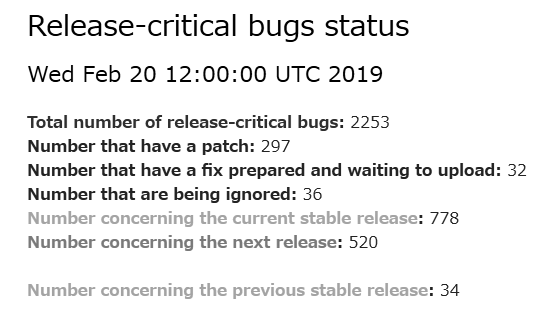
\includegraphics[width=0.45\hsize]{image201902/debian-rcbug-1_20190220_gray.png}
  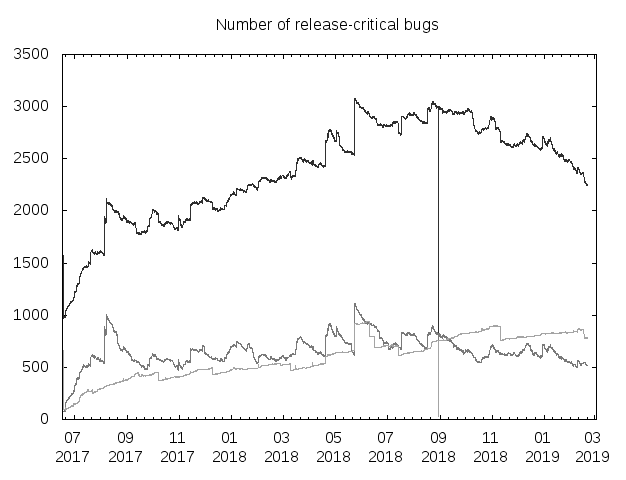
\includegraphics[width=0.45\hsize]{image201902/debian-rcbug-2_20190220_gray.png}
  % https://bugs.debian.org/release-critical/
\end{center}




\subsubsection{Debian 9 から 10 の変更点}


【ご注意ください】
この資料は2月現在のものです。リリースノート\footnote{\url{https://www.debian.org/releases/buster/amd64/release-notes/index.ja.html}}を参照してください。


usr-merge の完全適用は Buster では一部見送り

\begin{itemize}
\item \url{https://wiki.debian.org/UsrMerge}
\item /bin,/sbin,/libを、/usr/bin,/usr/sbin,/usr/lib へのシンボリックにすること
\item 一部のパッケージで問題が出たため、技術委員会も含めてBuster ではどうするか 議論になった
  \begin{itemize}
  \item 議論の結果、usr-merge の取り組みは Buster のリリース後に改めて進めことになった
  \item 「tech-ctte: Should debootstrap disable merged /usr by default?」 \url{https://bugs.debian.org/cgi-bin/bugreport.cgi?bug=914897}
  \item 「usrmerge -- plan B?」のスレッドを参照 \url{https://lists.debian.org/debian-devel/2018/11/msg00354.html}
  \end{itemize}
\end{itemize}




%\begin{frame}{Debian 9 から 10 の変更点}% [containsverbatim]
%
%secure boot
%  
%\begin{itemize}
%\item secure boot対応で問題となるバグはすべて解決済み
%\item 皆さんがお持ちのPCで試した動作結果の報告を募集しています
%  \begin{itemize}
%  \item \url{https://wiki.debian.org/SecureBoot/Testing}
%  \end{itemize}
%\end{itemize}
%    
%



linux kernelとglibcのバージョンアップに伴う変更
  
\begin{itemize}
\item apparmorはデフォルトで有効になる
\item Busterをコンテナ環境で動かす場合の制限
  \begin{itemize}
  \item glibc-2.26以降を採用しており、linux-3.2以降が必要
  \item ホスト側がとても古いサーバの場合に Buster がコンテナ環境で動かない場合あり
  \end{itemize}
\item Busterをホスト環境で動かす場合の制限
  \begin{itemize}
  \item amd64において、古い'virtual syscall' がデフォルトで無効
  \item glibc-2.13以下のシステムはコンテナ環境で動かない
    \begin{itemize}
    \item Debian-7以下、RHEL/CentOS-6 以下が該当
    \end{itemize}
  \item 有効にする場合はカーネルパラメータに vsyscall=emulate を追加
  \end{itemize}
\end{itemize}





GNOME は Wayland での動作がデフォルト

\begin{itemize}
\item 「GNOME on Xorg」も選べます
\item 他のデスクトップ環境は Xorg で動作します
\item GNOME で Wayland を使う場合に日本語を入力できないことがある
  \begin{itemize}
  \item 日本語入力処理(Input Method)周りに問題が残っており、修正対応中
  \end{itemize}
\end{itemize}

\begin{center}
  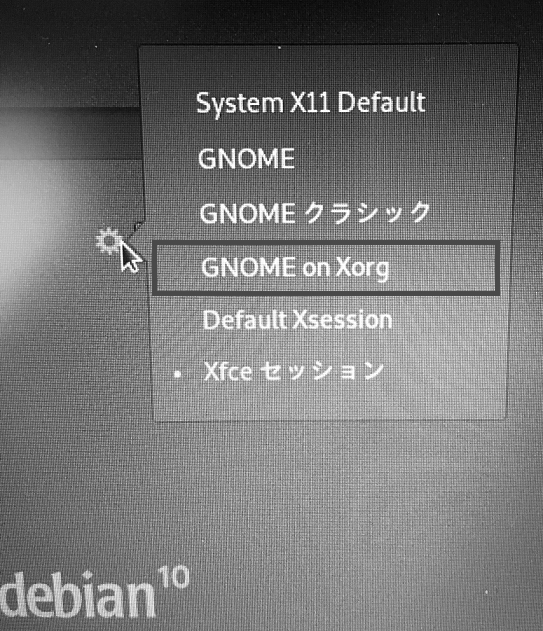
\includegraphics[width=0.5\hsize]{image201902/GDM_GNOME_select_mark_gray.png}
\end{center}





  \begin{itemize}
  \item openssl-1.1.1系の採用によりTLSv1.3が利用可能
  \item opensshにおいてSSH 1プロトコルが完全削除。SSH 2プロトコルを利用すること。
  \item Debian 10では、Debian 9と同じアーキテクチャをサポートする\footnote{2019年2月の本記事作成時にはサポートアーキテクチャはまだ確定していなかった。}
    \begin{itemize}
    % \item 参考:Debian 9でサポートしているアーキテクチャ
    \item amd64, i386(i686以降), armel, armhf, arm64, mips, mipsel, mips64el, ppc64el, s390x
    \end{itemize}
  \end{itemize}




\subsubsection{バグレポート}

  \begin{itemize}
  \item 何かおかしい動作や不具合を見つけた場合はバグレポートをお願いします
  \item バグレポートの仕方(レポートは英語で送る必要あり)
    \begin{itemize}
    \item \url{https://www.debian.org/Bugs/Reporting.ja.html}
    \end{itemize}
  \item バグレポートの前にちょっと相談してみたい方は、日本語のDebian JPメーリングリストや、SNSで相談してみてください
    \begin{itemize}
    \item \url{https://www.debian.or.jp/community/ml/openml.html}
    \item Twitter: @debian\_jp
    \end{itemize}
  \end{itemize}


%-----------------------

\subsection{Debian Updates}

% 半年間の以下MLから抜粋して紹介する
%  debian-announce@lists.debian.org
%  debian-devel-announce@lists.debian.org

  %\begin{center}\Huge{Debian Updates}\end{center}



\subsubsection{released timeline}


\begin{itemize}
  \item 2018/11/10:  Updated Debian 9.6  released
  \item 2019/01/23:  Updated Debian 9.7  released
  \item 2019/02/16:  Updated Debian 9.8  released
\end{itemize}




\subsubsection{Bits from the DPL}


Bits from the DPL

\begin{itemize}
\item 月に1回"debian-devel-announce@lists.debian.org"のMLにChrisさんがプロジェクトの進捗を報告している
\item 時間のない方でもこれを読んでおけばDebian Projectの大まかな動きがわかる
\end{itemize}

\small{
\begin{itemize}

\item 2018/10/31 \url{https://lists.debian.org/debian-devel-announce/2018/10/msg00005.html}
\item 2018/11/30 \url{https://lists.debian.org/debian-devel-announce/2018/11/msg00007.html}
\item 2018/12/31 \url{https://lists.debian.org/debian-devel-announce/2018/12/msg00006.html}
\item 2019/01/31 \url{https://lists.debian.org/debian-devel-announce/2019/01/msg00010.html}

\end{itemize}
}




\subsubsection{Rust}


\begin{itemize}
\item 2018/11/02: Rust now available on 14 Debian architectures \\
\ \\
  \small{Rustコンパイラのブートストラップがmips、mips64el、mipsel、powerpcspeでもできるようになった。\url{https://lists.debian.org/debian-devel-announce/2018/11/msg00000.html}}

\end{itemize}




\subsubsection{SSH restriction}


\begin{itemize}
\item 2018/11/10: incoming SSH restriction for *.debian.org \\
\ \\
  \small{debian.orgのドメインを持つ一部のホストにおいて、セキュリティの観点からdebian.orgのサーバからのみssh接続を受け付けるように設定を変更した。\url{https://lists.debian.org/debian-devel-announce/2018/11/msg00003.html}}

\end{itemize}




\subsubsection{CTTE vendor-specific patch}


\begin{itemize}
\item 2018/11/13: CTTE decision on vendor-specific patch series (bug \#904302) \\
\ \\
  \small{DPKGにあるベンダー固有パッチ機能(主に派生ディストリビューションのUbuntuなどが利用している)を継続利用するか利用を止めるか議論があった。議論の結果、Debian 10 Busterのリリース後は利用を止めるべきとの提案がされた。\url{https://lists.debian.org/debian-devel-announce/2018/11/msg00004.html}}

\end{itemize}




\subsubsection{GSoC2019}


\begin{itemize}
\item 2019/01/16: Google Summer of Code 2019\\
\ \\
\small{Google Summer of Code 2019で取り組むプロジェクトのwikiページが立ち上がった。応募の例は、プロジェクトの例は「Android SDK Tools in Debian」、「Continuous Integration for biological applications inside Debian」、「Debian PHP Packaging」、「New Contributor Wizard」「Reproducible Builds」など。\url{https://lists.debian.org/debian-devel-announce/2019/01/msg00007.html}}

\end{itemize}




%-----------------------

\subsection{日本語によるDebianの情報}


\begin{itemize}
  \item Debian JP Project \\
      \url{https://www.debian.or.jp}
  \item 東京エリアDebian勉強会\\
      \url{https://tokyodebian-team.pages.debian.net/}
  \item 関西Debian勉強会 \\
      \url{https://wiki.debian.org/KansaiDebianMeeting}
  \item Twitter \\
      \url{@debian_jp}
  \item  雑誌 Software Design 技術評論社発行 \\
    「Debian Hot Topics」、GPG関連の記事など(隔月連載)
\end{itemize}

%201907 tokyo
\dancersection{Buster デスクトップの日本語入力}{yy\_y\_ja\_jp}

Debian の日本語入力はuim-mozcがデフォルト\footnote{一部のアーキテクチャはuim-anthy}で、お好みでibusやfcitxなど、anthyやskkなども使えます。Stretch (9) までと同様に Buster (10) でもふつうに使えるように、im-configというパッケージで対応を行いました。

Debian は長らくGNOMEがデフォルトデスクトップです。Stretchでは図\ref{fig:desktop-stretch}のような感じでした。Busterでは図\ref{fig:desktop-buster}のようになり、あまり変わっていないように見えます。しかし、中身はかなり変わりました。

\begin{figure}[h]
\begin{center}
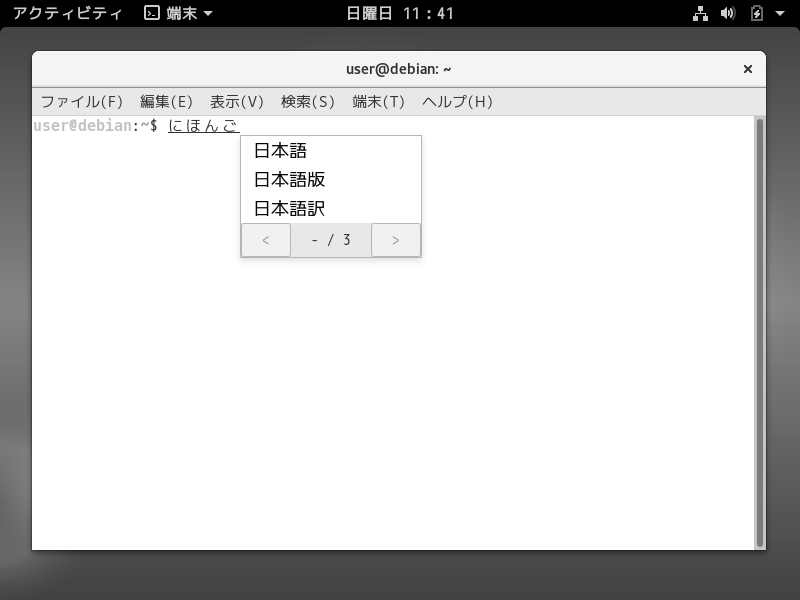
\includegraphics[keepaspectratio,width=0.45\hsize]{image201907/stretch_gnome_3_gray.png}
\end{center}
\caption{Stretch のデフォルトデスクトップ}
\label{fig:desktop-stretch}
\end{figure}

\begin{figure}[h]
\begin{center}
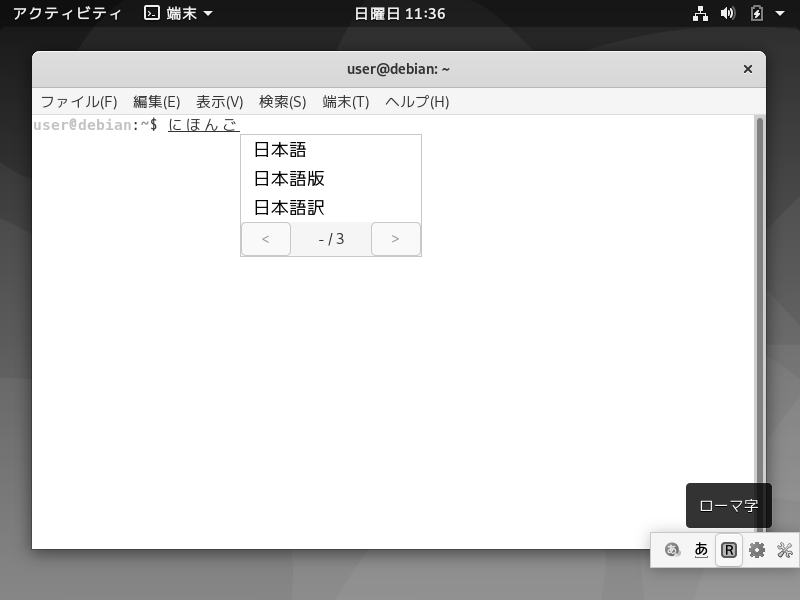
\includegraphics[keepaspectratio,width=0.45\hsize]{image201907/buster_gnome_3_gray.png}
\end{center}
\caption{Buster のデフォルトデスクトップ}
\label{fig:desktop-buster}
\end{figure}

特に変わったのはGNOMEで、StretchまではGNOME on Xorgがデフォルトでしたが、BusterではGNOME on Waylandがデフォルトになりました。
WaylandではXorgで行われていた設定が何もされないなど様々な問題がありましたが、基本的には使えるようにしました。

\subsection{デフォルトデスクトップ}
Debianインストーラのソフトウェア選択画面では複数のデスクトップ環境を選べますが(図\ref{fig:d-i-tasksel})、そのうち一番上にあるものがデフォルトデスクトップと呼ばれています。
なおこの画面で選べるデスクトップ環境は、Buster では LXQt が加わった以外は特に並び順も変わっていません。

\begin{figure}[h]
\begin{center}
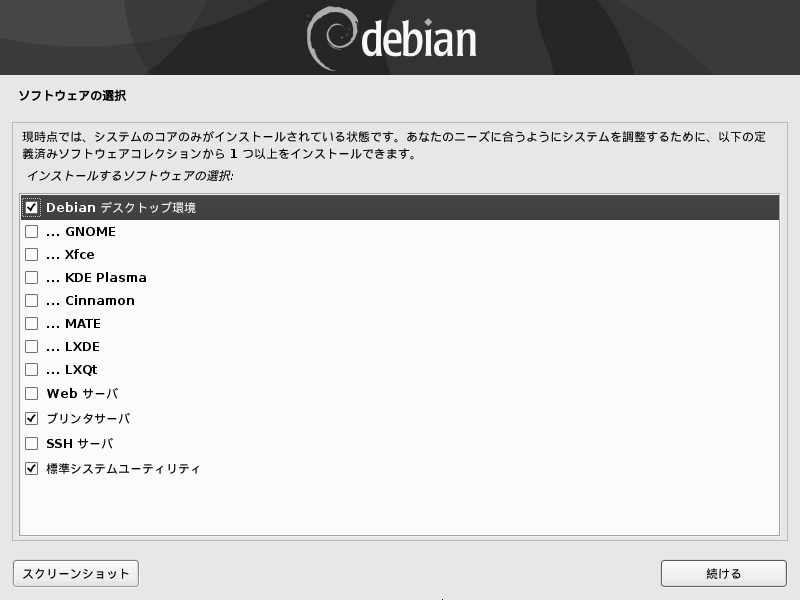
\includegraphics[keepaspectratio,width=0.7\hsize]{image201907/buster_tasksel_0_gray.png}
\end{center}
\caption{Debian インストーラのソフトウェア選択画面}
\label{fig:d-i-tasksel}
\end{figure}

ここでGNOMEにもチェックを入れて進むと、GNOMEデスクトップとともにログイン画面のディスプレイマネージャgdm3がインストールされます。

インストール完了後に起動するとgdm3のログイン画面になります。ユーザーを選択するとパスワード入力画面になりますが、ここでStretchのGNOMEから変わったところがあります。サインインボタンの左隣にある歯車をクリックすると、Stretch のログイン画面では図\ref{fig:gdm3-stretch}のように ``System X11 Default''が選択されており、また一番下のメニューは ``GNOME on Wayland''となっていました。しかしBusterでは図\ref{fig:gdm3-buster}のように一見Stretchのときにもあったようなメニューの ``GNOME'' が選択されており、また一番下のメニューが ``GNOME on Xorg''になっています。同じメニュー名 ``GNOME''でもStretchまでは実体がGNOME on Xorgでしたが、BusterのものはGNOME on Waylandになったのです。

\begin{figure}[h]
\begin{center}
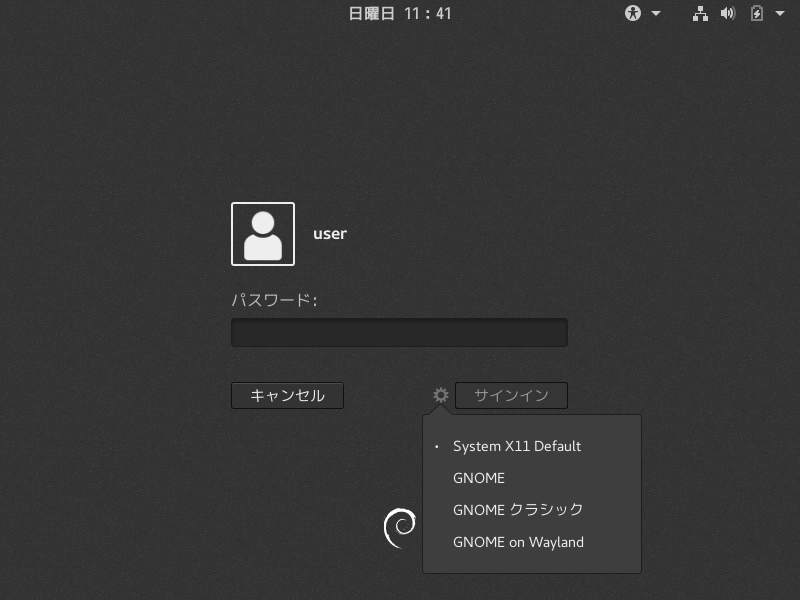
\includegraphics[keepaspectratio,width=0.7\hsize]{image201907/stretch_gnome_0_gray.png}
\end{center}
\caption{Stretch のログイン画面}
\label{fig:gdm3-stretch}
\end{figure}

\begin{figure}[h]
\begin{center}
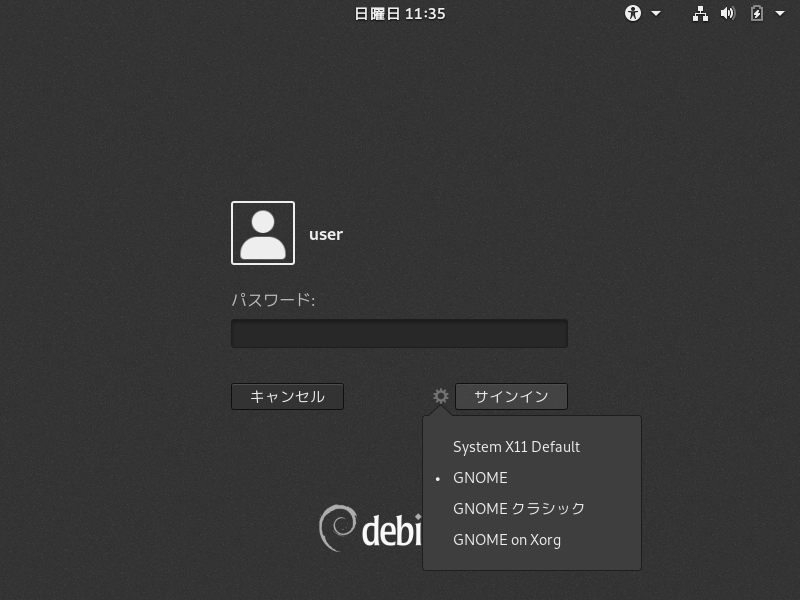
\includegraphics[keepaspectratio,width=0.7\hsize]{image201907/buster_gnome_0_gray.png}
\end{center}
\caption{Buster のログイン画面}
\label{fig:gdm3-buster}
\end{figure}

つまりデフォルトデスクトップがGNOMEであることは変わっていませんが、正確には

\begin{itemize}
 \item Stretch までは GNOME on Xorg
 \item Buster では GNOME on Wayland
\end{itemize}

となっています。

\subsection{Stretch までの im-config}
日本語などを入力するには入力メソッドフレームワークと入力メソッドエンジンの設定が必要です。この設定はGTK+やQtといったGUIライブラリ、もしくはXIM (X Input Method)に対して行う必要があり、例えばGTK+では\verb|GTK_IM_MODULE| といった環境変数が使われています。また、入力を変換するための補助ツールのデーモンや、入力メソッドの状態を表示するためのツールバーなどを起動する必要があります。
Debianには入力メソッドフレームワークがuim、ibus、fcitxなど複数あり、日本語環境のデフォルトはuimですがお好みで選ぶことができます。またDebianにはデスクトップもGNOMEに限らずたくさんあり自由に選べます。どのデスクトップを選んでも、そしてどの入力メソッドフレームワークを選んでも、インストールしたら何も触らなくてもデフォルトでこのような設定や起動がされるように、シェルスクリプトで書かれたim-configパッケージが自動設定してくれます。自動設定される値はインストールされているパッケージやログインユーザーの使う言語をもとに動的に変わります。なお、お好みでim-configを手動でユーザー毎やシステム全体に設定変更したり、im-configを使わずすべて手動で設定することもできるようになっています。

Stretchまでのim-configについて詳しくは2013年夏号の記事\footnote{\url{https://tokyodebian-team.pages.debian.net/pdf2013/debianmeetingresume2013-natsu.pdf}}をご覧ください。当時はWheezy (7.0)でしたが大きくは変わっていません。

%XXX config dependencies

\subsection{XIM と GUIライブラリ}
im-configはXIM関連で大きく2つの設定をしてきました。

1つ目はXIMへの設定、\verb|XMODIFIERS| 環境変数です。これは主にXIMで入力を直接扱う(GUIライブラリを使わない)アプリケーション、例えばxtermなど向けの設定ですが、2つ目の設定とも関連があります。

2つ目はGUIライブラリに対する設定です。uimなどの入力メソッドフレームワークはGUIライブラリそれぞれにプラグインを提供する必要があり、それがインストールされていればGUIライブラリは直接uimなどと通信できます。ただ、それがインストールされていなくてもGUIライブラリはXIMと通信する機能があります。GTK+の場合は\verb|GTK_IM_MODULE=xim|とすればXIMと通信します。1つ目の設定と組み合わせることで、GTK+はXIM経由でuimなどと通信することが可能です。

しかし、XIMによる入力は特定の条件でフリーズしたりとうまく動かないことがあることが知られていました。

\subsection{Stretch までの uim}
2017年冬号の記事 ``Debian Stretchのインプットメソッドの現状'' \footnote{\url{https://tokyodebian-team.pages.debian.net/pdf2017/debianmeetingresume2017-fuyu.pdf}}でも取り上げられていましたが、図\ref{fig:desktop-stretch}も見るとわかりますがStretchのGNOMEではuimの状態が画面上で見えません。KDEなどほかのデスクトップでも見えない、ないしわかりにくいものがありました。GNOMEやKDEなどデスクトップなどが変化していったことが原因かとみられます。

\subsection{GNOME}
DebianはWheezyでGNOME 3を取り込みましたが、それより前にあったGNOME 2とは大きく異なります。GNOME シェルというものを導入し、デスクトップでは標準的なシステムトレイを廃止してトップバー(画面最上部の黒いバー)に置き換えました。そのため今までシステムトレイに表示していたuimの状態は見えなくなってしまいました。そしてトップバーに表示するにはGNOME 3独自のJavaScript APIで描画しなければならず対応をむずかしくしています。

さらに、WheezyにはGNOME 3.4、Jessie (8) にはGNOME 3.14を含んでいましたが、バージョン3.5頃からGNOMEは入力メソッドフレームワークとしてibusを組み込みはじめたようで、GNOMEは独自D-Bus APIをibus専用に提供して通信しているようで、\verb|GTK_IM_MODULE|環境変数が設定されていなくてもGTK+でibusが動作するようです。ibus以外を使うこともできると記されてはいるものの、ibus-daemonが削除されていれば使えるとされています\urldef{\gnomeibusurl}\url{https://wiki.gnome.org/ThreePointFive/Features/IBus#How_to_use_other_IM_frameworks}\footnote{\gnomeibusurl}。つまりGNOMEでuimやfcitxなどibus以外を使うには、im-configなどの設定を切り替えるだけでなく、ibus-daemonというバイナリ(つまり \verb|/usr/bin/ibus-daemon|)を含んでいるibusパッケージを削除しないと動作保証されない、というモジュール化とは真逆の方向性で残念な状況です。実際、uimやfcitxの動作中にibusパッケージがインストールされたままだとibusを使っていないのにトップバーの表示がおかしくなったり、キー入力にibusが同時に反応したりということも起こったりするようです。

そして先ほど見たとおり、Stretchリリースより後に今までのXorgに代わりWaylandをデフォルトにしたようです\footnote{正確にはStretchに入っているGNOME 3.22でGNOME本家はWaylandデフォルトにしたものの、DebianはXorgデフォルトに戻していたようです(gnome-session 3.21.90-3)。Stretchがリリースされたので本家に合わせてWaylandデフォルトにしたようです。}。GNOME シェルは明らかにWaylandの場合に機能制限しています。GTK+にはウィンドウをAlt+Tabやタスクバーといったウィンドウ一覧に表示しないようにする設定\urldef{\gtktaskbarurl}\url{https://developer.gnome.org/gtk3/stable/GtkWindow.html#gtk-window-set-skip-taskbar-hint}\footnote{正確にはデスクトップ環境に対してタスクバーに表示しないよう要請する機能です。\\
\gtktaskbarurl}ができるのですが、Wayland上ではこの設定を無視します\footnote{\url{https://bugzilla.gnome.org/show_bug.cgi?id=771329}}。そのためGNOME on WaylandではツールバーウィンドウがAlt+Tab対象になってしまい入力しづらくなります。おそらくそんなツールバーなど廃止してしまってトップバー右側にでもGNOME 3独自のJavaScript APIで描画せよという主張なのでしょう。しかしそれでは他のデスクトップが困ります。

Wayland自体については後にまとめます。

\subsection{KDE}
DebianはStretchでKDE 5を取り込みました。uimにはシステムトレイのほかにKDE 4向けのPlasmaウィジェットがありますが、KDE 5では互換性がなく動作しません。

なおKDE 5にはkimpanelという入力メソッドの状態表示用Plasmaウィジェットが標準で組み込まれており、タスクバーの中にも最初から表示されています。fcitx開発者が作ったようで、fcitx-module-kimpanelパッケージをインストールすればfcitxの状態を表示できるようです。fcitx以外の入力メソッドフレームワークでもkimpanelのプロトコルで通信しさえすればkimpanelに状態表示できるようです。さらにこのkimpanelプロトコルを使ってGNOME 3でも状態表示すべくGNOME シェル拡張gnome-shell-extension-kimpanelパッケージを作ったようです。これを使えばGNOME 3独自の描画を入力メソッドフレームワークそれぞれが頑張らずに済むかもしれません。

またKDEもWayland対応を進めているようで、plasma-workspace-waylandパッケージをインストールすると試すことができます\footnote{後述しますが現時点ではこの上で起動されるアプリケーションはデフォルトXWaylandで動作しているようです。}。

\subsection{Wayland -- Xorg との違い}
Xorgは昔からありますが、Waylandは後発としてディスプレイサーバを一から作り直したようでさまざまな機能をおそらくあえて削っているようです。

\begin{itemize}
 \item セッションの初期化
 \begin{itemize}
  \item 環境変数などの設定
  \item デーモンなどの起動
 \end{itemize}
 \item ウィンドウの配置
 \begin{itemize}
  \item 位置情報の取得・設定
  \item 最前面表示など前後関係の設定
 \end{itemize}
\end{itemize}

Xorgの復習もしながら、それぞれの対策案もまとめます。

\subsubsection{セッションの初期化}
DebianのXorgでは、Xセッションは \verb|/etc/X11/Xsession| など\footnote{Debianのgdm3では \texttt{/etc/X11/Xsession} に似せた \texttt{/etc/gdm3/Xsession} が使われています。}から呼ばれる \verb|/etc/X11/Xsession.d/| などにあるシェルスクリプトで初期化されます。
シェルスクリプトなので環境変数などの設定もデーモンなどの起動もなんでもできます。
これらはgdm3などのディスプレイマネージャや\verb|startx|などのコマンドがXセッションを立ち上げるときに実行していました。
なお、\verb|~/.xsessionrc| などこれらのスクリプトが読み込んでくれるスクリプトを自分のホームディレクトリに置くことで自動設定から変更することもできますし、昔ながらの \verb|~/.xsession|など\footnote{これらも結局は \texttt{/etc/X11/Xsession.d/} から起動されています。}を置いてカスタマイズすることもできます\urldef{\startingxurl}\url{https://www.debian.org/doc/manuals/debian-reference/ch07.ja.html#_starting_the_x_window_system}\footnote{\startingxurl}。

入力メソッド周りの設定・起動はim-configパッケージのスクリプトが2段階に分けて行ってきました。
\begin{itemize}
 \item 1段階目(シェル変数 \verb|IM_CONFIG_PHASE| が \verb|1| のとき)は \verb|/etc/X11/Xsession.d/| に置かれている\\
 \verb|/etc/X11/Xsession.d/70im-config_launch|\footnote{70という大きめの番号にすることで、これより前で \texttt{\~{}/.xsessionrc}などのカスタマイズファイルが読まれるようにしてあります。}で、環境変数などの設定を行います。
 \item 2段階目(\verb|IM_CONFIG_PHASE| が \verb|2| のとき)が \verb|/usr/bin/im-launch| でデスクトップを起動する直前に実行され\footnote{このタイミングで実行されるように \texttt{/etc/X11/Xsession.d/70im-config\_launch} が仕込んであります。}、デーモンなどの起動をしてきました。
\end{itemize}
なお途中で前述の \verb|~/.xsessionrc| なども読まれているので、ホームディレクトリにあるそれらでカスタマイズされていればそれらが尊重されて設定・起動されます。

しかし、Waylandセッションは \verb|/etc/X11/Xsession.d/| を見ないのは当然とはいえ、何も初期化を扱いません。gdm3やKDEと同時にインストールされるsddmといったディスプレイマネージャはXセッションとWaylandセッション両方へのログインに対応していますが、どれもXセッションを立ち上げるときだけ上のような共通の初期化を行うようになっており、Waylandセッションでは何もしていません。なお\verb|startx|のようにディスプレイマネージャを使わずコマンドラインからWaylandセッションを起動する汎用の方法も用意しないようです。各デスクトップのWaylandセッションを独自にコマンドライン起動することはできるようですが\footnote{GNOME on Waylandセッションは \texttt{env XDG\_SESSION\_TYPE=wayland dbus-run-session gnome-session} で起動できるようです。}、その場合もそのデスクトップ独自の初期化以外はされません。そのため何らかのほかの汎用的な方法で初期化する必要があります。一方で``汎用的な方法''を単に採用すると、汎用的である以上WaylandセッションだけでなくXセッションでもその初期化が実行されてしまう、つまりXセッションでは二重に初期化されてしまうことになるので、
\begin{itemize}
 \item 二重に初期化されても(ほぼ)同じ結果になるようにする
 \item 今までのXセッションの方法を捨てて全部新たな方法で初期化する
\end{itemize}
など何らかの方法で対処しなければなりませんが、後者はほぼ完全互換でない限り困る人が多く非現実的です。

\paragraph{環境変数などの設定}
``汎用的な方法''はいくつか考えられますが、それぞれ課題があるので見ていきます。

\begin{itemize}
 \item \verb|/etc/profile.d/| にシェルスクリプト(\verb|*.sh|)を置く\\
このディレクトリは \verb|/etc/profile| から読み込まれます。この \verb|/etc/profile| は本来(コマンドライン)ログインシェル起動時に読み込まれるものですが、gdm3 や sddm では独自に読み込んでいます。そのため、これらのディスプレイマネージャではここに置けば設定はされます\footnote{実際Ubuntuのim-configはWaylandでなんとか動かすため\texttt{/etc/profile.d/input-method-config.sh}を仮置きしていたようです。}が、あらゆるコマンドライン端末などで余計な環境変数設定作業が行われてしまうことになるので避けられるなら避けたいところです。なお、Xfce などほかのデスクトップと同時にインストールされる lightdm などのディスプレイマネージャでは(少なくともBuster時点では)読み込まれないので、今までのXセッションの方法を完全に置き換えるまではできません。
 \item \verb|systemd --user| 独自空間の変数を設定する\\
DebianではJessieからsystemdが標準のinitシステムです。systemdではユーザー毎にログイン直後に\verb|systemd --user|というプロセスが立ち上がり、その内部で環境変数とは別に独自の変数を持っています\footnote{\texttt{systemctl --user show-environment}で中身が見られます。}。Stretchリリースよりも後の最近のsystemd(バージョン233以降)ではこの変数を静的・動的に設定できるようになりました。\verb|/etc/environment.d/*.conf| や \verb|~/.config/environment.d/*.conf| に \verb|KEY=VALUE| と書いておくと、\verb|KEY|という変数名に\verb|VALUE|という値が設定されます。動的に設定するには、\verb|/usr/lib/systemd/user-environment-generators/| 以下に \verb|KEY=VALUE| といった行を生成して出力するプログラムをシェルスクリプトでもなんでも置くことでできます。

さて、この独自変数を設定したところでこれは環境変数ではありません\footnote{\url{https://github.com/systemd/systemd/pull/3904} で当初は環境変数を設定する機能にしたかったようですが、セキュリティ上の懸念から独自変数を設定するだけの機能としてsystemd 233に追加されたようです。}。ここで現状gdm3だけはこの独自変数の値を環境変数として取り込むようになっており、デフォルトデスクトップとともにインストールされるgdm3\footnote{なおgdm3は\texttt{systemd --user}を使うためにsystemdに強く依存しているので、sysvinitなどsystemd以外のinitでは使えません。}に限っていえば環境変数の動的設定に使えそうです。それ以外では使えないですから当然今までのXセッションの方法を完全に置き換えるまではできません\footnote{sysvinitなどsystemd以外のinit上でsystemd-logind相当の機能を使えるようにするelogindパッケージがありますが、\\
\texttt{systemd --user}相当の機能はなく、提供の予定もありません。}。

また、この \verb|systemd --user| プロセスはデスクトップセッションとは独立しており、例えば同じユーザーでコンソールログインしたりするとそのプロセスは共有されます。そのためデスクトップをログアウトしても終了しないことがあります。また、同じユーザーがすべてログアウトしたとしても少なくともしばらくの間は生き続けるようです。つまり設定を変更して再ログインしてもプロセスが変更前の設定を覚えたままになっていることがあるので、他人と同時利用しないPCであればログアウトだけでなく再起動するのが確実です。

そしてこのプロセスはデスクトップセッションと独立していることから、設定時にはどのデスクトップでログインしようとしたのかすらわかりません。XorgなのかWaylandなのか、はてはSSHログインなのかも区別できないので、今までのXセッションの方法を維持するならXorg上で二重設定を回避できません。

なお今までのXセッションの方法にも悪影響があります。もともとXセッションの方法ではほぼまっさらの未設定の状態で設定を行っていました。しかし、この \verb|systemd --user| プロセスはログイン直後の非常に早いタイミングで起動されるので、この初期化よりも後に今までのXセッションの方法による初期化が行われることになり、既に \verb|systemd --user| により設定済みの上に \verb|~/.xsessionrc| などユーザーによるカスタマイズも含むXセッションの方法による初期化を行うことになってしまいます。何らかの対処が必要です。
 \item \verb|pam_env(7)|で使われる変数を設定する\\
\verb|pam_env.so|はPAM (Pluggable Authentication Module)という認証フレームワークのモジュールで、ディスプレイマネージャ、コンソール、SSHサーバなどでのログイン認証時に環境変数を設定してくれるものです。\verb|/etc/environment| などに \verb|KEY=VALUE| と書いておくと、このモジュールから読み込まれれば環境変数\verb|KEY|が\verb|VALUE|に設定されます。しかしこのモジュールはおそらくセキュリティ上の懸念からかDebianではデフォルトではあまり使わないようになっており、ホームディレクトリに \verb|~/.pam_environment|を置けば読み込んでくれる機能もあるのですがデフォルトではsddmでのみ使われています\footnote{\texttt{/etc/pam.d/} 内の設定ファイルで\texttt{pam\_env.so}の行に\texttt{user\_readenv=1}と書く必要があります。Ubuntuのgdm3では有効になっているようです。}。また、これらの設定ファイルには静的な決まった値しか書けません。設定を動的に変える機能がほぼないため\footnote{\texttt{pam\_env.conf(5)} で他の変数からの展開ができるくらいです。}im-configには使えません。\verb|pam_env.so|を改造した動的に入力メソッド周りを設定するモジュールを作ろうと思えば作れるでしょうが、そこまで複雑なことを認証フレームワークのモジュールでやるのはやり過ぎでしょう。
 \item (参考)ディスプレイマネージャやデスクトップ独自の設定ファイルを使う\\
例えばgdm3は \verb|/etc/xprofile|や \verb|~/.xprofile|などを、GNOMEは \verb|~/.gnomerc|を独自に読み込むようで、ここに挙げたものはどれもシェルスクリプトなので動的に設定できるようです。ただどれも汎用的でないので可能な限り避けたいところです。
\end{itemize}

\paragraph{デーモンなどの起動}
こちらの``汎用的な方法''は1つくらいしかありません。デスクトップ環境に共通の仕様を提供しているfreedesktop.orgという団体が定めるXDG Autostart\footnote{\url{https://standards.freedesktop.org/autostart-spec/autostart-spec-latest.html}}という仕組みで、現代的なデスクトップ環境(GNOME、KDE、Xfceなど)は対応しており自動起動設定に使われています。\verb|.desktop| という拡張子の``デスクトップファイル''\footnote{これもfreedesktop.orgが定めています。\url{https://specifications.freedesktop.org/desktop-entry-spec/latest/}}を \verb|/etc/xdg/autostart/| や \verb|~/.config/autostart/| に置いておくと、XDG Autostart対応デスクトップのログイン直後に起動されます。なお非対応のデスクトップでは使えないので、やはりこれで今までのXセッションの方法を完全に置き換えるまではできません。なお今までのXセッションの方法を維持するならXorg上で二重起動しないようにする必要があります。

% \paragraph{まとめ}
% ここまで見てきたさまざまな設定・起動方法を図\ref{fig:config-deps}に示します。
% %\begin{sidewaysfigure}[h]
% \begin{figure}[h]
% \centering
% \begin{center}
% \includegraphics[keepaspectratio,width=1\hsize]{image201907/env-config.png}
% \end{center}
% \caption{さまざまな設定・起動方法}
% \label{fig:config-deps}
% \end{figure}
% %\end{sidewaysfigure}

\subsubsection{ウィンドウの配置}
\paragraph{位置情報の取得・設定} Xorgではウィンドウなどの位置情報を取得したり、指定した位置にウィンドウを配置することができました。しかしWaylandはそのような機能を提供しません。今あるカーソルの位置もわからないので、入力メソッドフレームワークが変換候補を表示しようとしてもカーソルの近くに出せません。ツールバーウィンドウを右下の決まった位置に置いたりすることもできません。

\paragraph{最前面表示など前後関係の設定} Xorgではウィンドウを最前面に固定したりすることができましたが、Wayland自体にはそのような機能がありません。そのためツールバーウィンドウを最前面にできないので、例えばエディタのウィンドウを画面全体に最大化するとツールバーは隠れてしまい状態が見えなくなってしまいます。

\paragraph{対策案} どちらも解決するために次のような方法が考えられます。
\begin{itemize}
 \item Waylandコンポジター(GNOME シェル\footnote{正確にはmutter}など)の独自APIで実装する\\
       Waylandではコンポジターというディスプレイサーバーが表示します。コンポジターはさまざまなアプリケーションの複数のウィンドウを適切に配置したり最前面にしたりしていますし、ウィンドウのメニューから手動で指定さえできるようにしてあるわけなので、Wayland自体にAPIがなくてもコンポジターがAPIを提供していればそれを使えるはずです\footnote{ただし標準にならない限りコンポジター(つまりデスクトップ)毎に独自APIばかりになってしまうでしょう。}。
ibusはGNOMEに組み込まれているためこの方法を使っていますが、ほかの入力メソッドフレームワーク向けにGNOMEがこのAPIを公開するつもりはなさそうなので、この方法は現状ibus以外では使えません。
 \item XWayland を使う\\
Waylandコンポジター内でXWaylandというXサーバを動かすことができます。このXWaylandの中では普通のXアプリケーションを動かすことができ、普通のXorgのように位置の取得や設定、最前面設定などができるようです。なお普通のXorgと同様なので、GNOMEのタスクバー非表示も機能します。GTK+やQtはこの切り替えに対応しており、環境変数さえ設定すれば簡単に切り替えられるようです。GTK+アプリケーションの場合は\verb|env GDK_BACKEND=x11| でプログラムを起動すればXWayland内で表示されます\footnote{Qtアプリケーションの場合は\texttt{env QT\_QPA\_PLATFORM=xcb} ですが指定していなくても現状はXorg (XWayland)が標準のようで、Waylandにしたいときは\texttt{env QT\_QPA\_PLATFORM=wayland}とします。}。
\end{itemize}

\subsection{Buster の im-config}
ここまで見てきた対策案を踏まえて、Busterのim-config (0.43-1)では次のようにすることにしました。

まず、結局今までのXセッションの方法を完全に置き換えられるような互換性高い方法は存在しないので、Xorgでは今まで通り設定や起動をすることにします。

そしてWayland(Xorg以外)向けには\verb|systemd --user| の独自変数を設定し\footnote{\texttt{/usr/lib/systemd/user-environment-generators/70-im-config}}、XDG Autostartを使ってWaylandデスクトップのときだけ\footnote{XDG Autostartのデスクトップファイル内ではどんなディスプレイサーバやデスクトップで実行されているかの情報が環境変数で取得できます。Waylandでは\texttt{XDG\_SESSION\_TYPE} 環境変数が \texttt{wayland} になります。}起動することにします\footnote{\texttt{/etc/xdg/autostart/im-launch.desktop}}。しかしこのままだとXorgで二重設定になってしまいます。また、ユーザーがカスタマイズしたスクリプトでデーモンを起動していたりすると二重起動になってしまいます。二重設定は諦めざるを得ませんが、ユーザーがカスタマイズした設定を尊重して可能な限り二重起動されないように試みます。具体的には、\texttt{systemd --user}が最初に起動されるのは回避不可能なので、それより後に実行されるXセッションでの起動時に
\begin{itemize}
 \item (\verb|systemd --user| や \verb|~/.xessionrc|などにより)先に設定された設定値
 \item まっさらな未設定にした状態で、今までのim-configで初期化し、それによる設定値
\end{itemize}
の2つを比較することで、少なくともユーザーがデフォルトとは異なる値にカスタマイズしようとしていたかを判定します\footnote{\texttt{/usr/bin/im-launch}の \texttt{IM\_CONFIG\_CHECK\_ENV} の部分でこのようなちょっと複雑なことをしています。}。異なる値が見つかった場合は明らかにカスタマイズされているということなのでim-configでの起動を行いません。ただ、見つからなかった場合でもたまたまim-configが設定しようとした値と同じ値をユーザーがカスタマイズした設定ファイルで設定していたかもしれませんが、これを知る方法はないのでそのような場合は二重起動になります。自分で入力メソッド周りの設定スクリプトを書いている方は、二重起動などに遭遇したら一度自分の設定を削ってみて試していただきたいです。

また、XWaylandでツールバーなどを起動することにします。今のところuimのツールバーはXWaylandを使うようにしました\footnote{実はfcitxは調べきれてませんが何らかの方法で問題を回避してツールバーを表示しているようです。}。

また、GNOME は ibus-daemon が存在すると起動していなくても衝突することから、残念ながら ibus-daemon が存在するときは Xorg以外の環境の im-config は何も設定・起動しないようにしました。つまりWaylandでibusパッケージがインストールされているとim-configは動作しないようになります。なおこれは本当はGNOMEの問題ですが、\verb|systemd --user|の設定時はデスクトップの種類がまったくわからないため、そして今のところXorg以外でまともに動作するデスクトップはGNOMEだけなので、Xorg以外では常に何もしないようにしてあります\footnote{GNOMEの問題なので実はGNOME on Xorgでも発生し得る問題ですが、互換性のためXorgでの挙動は変えていません。}。

また、XIMでは入力に問題が起きることがあることから、GUIライブラリがXIM経由で入力メソッドフレームワークと通信するのを止めました。つまり入力メソッドフレームワークのGUIライブラリプラグインをすべてインストールしていないと、未インストールのGUIライブラリを使ったアプリでは入力できなくなります\footnote{uimを使うにはuimパッケージを推奨パッケージ(Recommends)まですべてインストールするようにしてください。なおDebianインストーラで普通にインストールすればこの状態になります。}。なおこれは、\verb|systemd --user|はディスプレイマネージャであってもSSHサーバであってもあらゆるログイン時に起動されるため、im-configの設定に時間が掛かりすぎて問題になってしまったための回避策でもあります\footnote{\url{https://bugs.debian.org/925160}}。

何か問題を見つけたらぜひim-configパッケージにバグレポートをお願いします\footnote{もちろん勉強会やTwitter、メーリングリストなどで教えていただいても構いません。}。

\subsection{Buster の uim}
Stretchではデフォルトで状態表示できていなかったので、Busterのuimは図\ref{fig:desktop-buster}のようにデフォルトでツールバーを表示するよう改修されました。なお、Stretchリリースより後にuimはWayland対応されたのですが、GNOME \verb|<del>|による嫌がらせ\verb|</del>| やWayland自体のせいで入力するのが難しい状態なので、im-configから起動されるときに \verb|env GDK_BACKEND=x11| を設定することで常にXorgないしXWaylandで動作するようにしてあります。

\subsection{今後}
いくつも課題があります。
\begin{itemize}
 \item 例えばKDE Plasma Waylandでは現状日本語入力できません。デフォルトになってしまったGNOME on Waylandに限ってはsystemdかつgdm3で日本語入力できるようにしましたが、KDEともにインストールされるsddmなどが何らかの汎用的な方法で環境変数などを設定できるようになる必要があります。本当はfreedesktop.orgなどの団体が特定のデスクトップやinitシステムなどに依存しない設定のための標準仕様を提供してくれるのが望ましいです\footnote{Waylandは何もないから困っているわけですが、実はXorgでもDebianは \texttt{/etc/X11/Xsession.d/} を使っているものの、設定方法はある程度似通った部分はあるもののディストリビューション毎にまちまちだったりします。}。
 \item 最近ではflatpak\footnote{flatpakというDebianパッケージをインストールするとflatpakパッケージを扱えるようにはなります。}やsnap\footnote{Ubuntuはデフォルトですが、snapdというDebianパッケージをインストールするとsnapパッケージを扱えるようにはなります。}といったコンテナでアプリケーションをパッケージ化する技術が増えてきていますが、日本語入力ができません。これはホスト側(手元のマシン)にある入力メソッドのデーモンなどとゲスト側(コンテナ内)にあるアプリケーションが通信できないからです。最近のflatpakではibusがGNOMEとの間で使っているD-Bus通信をできるようにコンテナに穴を開けているらしいですが、ibus以外の入力メソッドフレームワークもibusと同じD-Bus APIで通信しなければならないという流れでしょうか。しかしそのAPIをGNOMEは公開するつもりがありません。困りました。ただ、今まではGNOMEとibusだけで知っていたAPIをflatpakプロジェクトにも教えたということであれば、ほかで同じAPIを勝手に使ったとしてもそんなに頻繁にはAPIが変更されないことは期待できそうな気がします。
 \item GTK+4など新しいGUIライブラリが出てきたら対応はいつも必要です。GTK+4についてはGTK+3までと同じ環境変数\verb|GTK_IM_MODULE|が使えるようです。なおこれはGUIライブラリに限らずWaylandなどのディスプレイサーバやコンテナについても同じことが言えます。
 \item そもそも環境変数を使っているとコンテナなどいろいろな環境への情報伝搬が難しくなっています。ibusとGNOMEとの独自D-Bus APIが最良なのかはわかりませんが、他の標準的な方法でも通信できるようになると良いのかもしれません\footnote{もともとXIMも共通プロトコルだったような気はしますが...}。
\end{itemize}

\subsection{まとめ}

BusterではGNOME on Waylandがデフォルトデスクトップになりましたが、im-configに手を入れてなんとか日本語入力できるようにしました。またuimの課題もいくらか修正されています。Debianはさまざまなデスクトップや入力メソッドフレームワークを自由に選べます。im-configは、どのデスクトップを選んでも、そしてどの入力メソッドフレームワークを選んでも、インストールしたら何も触らなくてもデフォルトで設定・起動してくれる支援パッケージです。Waylandでは標準的な環境設定方法があまりないため、今回デフォルトデスクトップであるsystemd + gdm3 + GNOME Waylandの組み合わせについては\verb|systemd --user|の独自変数とXDG Autostartを使って動作するようにしました。KDE Plasma WaylandなどのWayland環境や、flatpak、snapといったコンテナ環境、今後出てくるだろうGUIライブラリなどでも自由に選んでそのままで使える状態にするのが課題です。

%201905 
%-------------------------------------------------------------------------------
\dancersection{/usr Mergeについて}{yy\_y\_ja\_jp}
%-------------------------------------------------------------------------------

Debian では Buster から ``/usr Merge'' がデフォルトになりそうです。概要と状況を整理します。

\subsection{概要}

``/usr Merge'' とは、\verb|/bin/|, \verb|/sbin/|, \verb|/lib/| などの中にあるもの(バイナリ等)を \verb|/usr/| 内に移す、つまり \verb|/usr/| 内にバイナリ等をすべて統合することです。
例えば \verb|/bin/ls| を \verb|/usr/bin/ls| に移します。また、今まで通り \verb|/bin/ls| でも使えるように互換性のため \verb|/bin| は \verb|/usr/bin| へのシンボリックリンクにします。\verb|/sbin| なども同様です。

なお、このような構成にしたい理由はsystemdのwiki\footnote{\url{https://www.freedesktop.org/wiki/Software/systemd/TheCaseForTheUsrMerge/}}などにまとめられているようです
\footnote{Debian wiki \url{https://wiki.debian.org/UsrMerge}}。

Debianを新規インストールするときには、Debianインストーラが内部で実行するdebootstrapがこの構成を行います。既存のDebian環境にはusrmergeパッケージをインストールすればこの構成にしてくれます\footnote{Busterの次のバージョンBullseyeではインストール推奨となるかもしれません。\url{https://bugs.debian.org/841666}}。なお、以前の構成へ元に戻すことは困難です。

Stretch インストーラで作った Debian 環境の \verb|/| 直下は次のようなディレクトリ構成でした。
\begin{commandline}
$ ls -l /
合計 76
drwxr-xr-x  2 root root  4096  5月 14 00:42 bin
drwxr-xr-x  3 root root  4096  5月 14 00:43 boot
drwxr-xr-x 17 root root  2980  5月 14 00:56 dev
drwxr-xr-x 76 root root  4096  5月 14 00:56 etc
drwxr-xr-x  3 root root  4096  5月 14 00:43 home
lrwxrwxrwx  1 root root    29  5月 14 00:38 initrd.img -> boot/initrd.img-4.9.0-9-amd64
lrwxrwxrwx  1 root root    29  5月 14 00:38 initrd.img.old -> boot/initrd.img-4.9.0-9-amd64
drwxr-xr-x 15 root root  4096  5月 14 00:42 lib
drwxr-xr-x  2 root root  4096  5月 14 00:36 lib64
drwx------  2 root root 16384  5月 14 00:35 lost+found
drwxr-xr-x  3 root root  4096  5月 14 00:35 media
drwxr-xr-x  2 root root  4096  5月 14 00:35 mnt
drwxr-xr-x  2 root root  4096  5月 14 00:35 opt
dr-xr-xr-x 80 root root     0  5月 14  2019 proc
drwx------  2 root root  4096  5月 14 00:35 root
drwxr-xr-x 14 root root   460  5月 14 00:57 run
drwxr-xr-x  2 root root  4096  5月 14 00:56 sbin
drwxr-xr-x  2 root root  4096  5月 14 00:35 srv
dr-xr-xr-x 13 root root     0  5月 14 00:57 sys
drwxrwxrwt  8 root root  4096  5月 14 00:56 tmp
drwxr-xr-x 10 root root  4096  5月 14 00:35 usr
drwxr-xr-x 11 root root  4096  5月 14 00:35 var
lrwxrwxrwx  1 root root    26  5月 14 00:38 vmlinuz -> boot/vmlinuz-4.9.0-9-amd64
lrwxrwxrwx  1 root root    26  5月 14 00:38 vmlinuz.old -> boot/vmlinuz-4.9.0-9-amd64
$ 
\end{commandline}

一方、Buster インストーラで作った Debian 環境では次のようになります。なお、現時点ではインストーラに ``/usr Merge'' しないようにする設定はなさそうです\footnote{\url{https://bugs.debian.org/923091}}。
\begin{commandline}
$ ls -l /
合計 60
lrwxrwxrwx  1 root root     7  5月 14 00:36 bin -> usr/bin
drwxr-xr-x  3 root root  4096  5月 14 00:43 boot
drwxr-xr-x 17 root root  3160  5月 14 00:56 dev
drwxr-xr-x 67 root root  4096  5月 14 00:56 etc
drwxr-xr-x  3 root root  4096  5月 14 00:43 home
lrwxrwxrwx  1 root root    30  5月 14 00:38 initrd.img -> boot/initrd.img-4.19.0-4-amd64
lrwxrwxrwx  1 root root    30  5月 14 00:38 initrd.img.old -> boot/initrd.img-4.19.0-4-amd64
lrwxrwxrwx  1 root root     7  5月 14 00:36 lib -> usr/lib
lrwxrwxrwx  1 root root     9  5月 14 00:36 lib32 -> usr/lib32
lrwxrwxrwx  1 root root     9  5月 14 00:36 lib64 -> usr/lib64
lrwxrwxrwx  1 root root    10  5月 14 00:36 libx32 -> usr/libx32
drwx------  2 root root 16384  5月 14 00:36 lost+found
drwxr-xr-x  3 root root  4096  5月 14 00:36 media
drwxr-xr-x  2 root root  4096  5月 14 00:36 mnt
drwxr-xr-x  2 root root  4096  5月 14 00:36 opt
dr-xr-xr-x 79 root root     0  5月 14  2019 proc
drwx------  2 root root  4096  5月 14 00:36 root
drwxr-xr-x 15 root root   460  5月 14 00:58 run
lrwxrwxrwx  1 root root     8  5月 14 00:36 sbin -> usr/sbin
drwxr-xr-x  2 root root  4096  5月 14 00:36 srv
dr-xr-xr-x 13 root root     0  5月 14 00:56 sys
drwxrwxrwt  8 root root  4096  5月 14 00:56 tmp
drwxr-xr-x 13 root root  4096  5月 14 00:36 usr
drwxr-xr-x 11 root root  4096  5月 14 00:36 var
lrwxrwxrwx  1 root root    27  5月 14 00:38 vmlinuz -> boot/vmlinuz-4.19.0-4-amd64
lrwxrwxrwx  1 root root    27  5月 14 00:38 vmlinuz.old -> boot/vmlinuz-4.19.0-4-amd64
$ 
\end{commandline}

\subsection{経緯}

``/usr Merge'' は以前Fedoraで特に行われていたようです\footnote{\url{https://fedoraproject.org/wiki/Features/UsrMove}}。なおFedoraは必須化したようです。

Debianでは当初Stretchでデフォルトにする予定でしたが、問題の解決が間に合いそうになく延期されました\footnote{\url{https://lists.debian.org/debian-devel-announce/2017/01/msg00004.html}}。

その後Busterに向けてdebootstrap 1.0.102で再度デフォルトにすることにしました\footnote{\url{https://bugs.debian.org/839046}}が、問題があるためデフォルトでなくすべきではという議論があり、Debian技術委員会(tech-ctte)にも持ち込まれました\footnote{\url{https://bugs.debian.org/914897}}。

%
Debian技術委員会は、debootstrapのメンテナーが決めたことは覆さない、
%つまり強権発動はしない
と決定しました\footnote{\url{https://lists.debian.org/debian-devel-announce/2019/03/msg00001.html}}。
同時に、Debianにおける``/usr Merge''の現状と今後の望ましい姿を示しました。

\subsection{現状}
Debian技術委員会の決定により、debootstrapメンテナー次第で``/usr Merge''がデフォルトになるかどうかは決まります。現時点で testing (Buster) 以降のバージョン向けにdebootstrapを実行すると次のようになっており、メンテナーが変更しなければこのままBusterリリースとなります。

\begin{itemize}
 \item 通常の環境では``/usr Merge''がデフォルト有効(無効にするには \verb|--no-merged-usr|オプションを付ける)
 \item パッケージビルド用の環境(\verb|--variant=buildd| オプション)ではデフォルト無効
\end{itemize}

なお、現状では``/usr Merge''された環境でビルドされたバイナリパッケージを``/usr Merge''されていない環境に持っていくと動作しないものがあり、それらのパッケージに随時バグ報告してくれている方がいるようです\footnote{\url{https://bugs.debian.org/cgi-bin/pkgreport.cgi?tag=usrmerge;users=md@linux.it}}
。よくある理由としては、ビルド中にバイナリの場所を \verb|/bin/| の中よりも先に \verb|/usr/bin/| を探しに行き、``/usr Merge''された環境では \verb|/usr/bin/| のパスをコンパイル結果に埋め込むからです。
例えば quilt パッケージの少し古い修正\footnote{\url{https://bugs.debian.org/913226}}以前のバージョン 0.65-2 を``/usr Merge''された環境でビルドしてみます。\verb|dh_auto_configure| 経由で実行された \verb|./configure| が \verb|/bin/bash| ではなく \verb|/usr/bin/bash|、\verb|/bin/cp| ではなく \verb|/usr/bin/cp|、などを検出してビルドしています。
この場合はビルドされたパッケージ内のシェルスクリプトの先頭が \verb|#! /usr/bin/bash| となったため lintian がたまたま別件のポリシー違反として検出してくれています。
\begin{commandline}
$ dget http://snapshot.debian.org/archive/debian/20180809T030926Z/pool/main/q/quilt/quilt_0.65-2.dsc
dget: retrieving http://snapshot.debian.org/archive/debian/20180809T030926Z/pool/main/q/quilt/quilt_0.65-2.dsc
(snip)
quilt_0.65-2.dsc:
      Good signature found
   validating quilt_0.65.orig.tar.gz
   validating quilt_0.65-2.debian.tar.xz
All files validated successfully.
dpkg-source: info: extracting quilt in quilt-0.65
(snip)
dpkg-source: info: applying fix-mail-threading
$ cd quilt-0.65/
$ debuild -us -uc
 dpkg-buildpackage -us -uc -ui
dpkg-buildpackage: info: source package quilt
dpkg-buildpackage: info: source version 0.65-2
(snip)
dh_auto_configure -- --with-docdir=/usr/share/doc/quilt --with-sendmail=/usr/sbin/sendmail --with-awk=/usr/bin/awk
  ./configure --build=x86_64-linux-gnu --prefix=/usr --includedir=\${prefix}/include --mandir=\${prefix}/share/man 
  --infodir=\${prefix}/share/info --sysconfdir=/etc --localstatedir=/var --disable-silent-rules 
  --libdir=\${prefix}/lib/x86_64-linux-gnu --libexecdir=\${prefix}/lib/x86_64-linux-gnu --runstatedir=/run 
  --disable-maintainer-mode --disable-dependency-tracking --with-docdir=/usr/share/doc/quilt 
  --with-sendmail=/usr/sbin/sendmail --with-awk=/usr/bin/awk
configure: WARNING: unrecognized options: --disable-silent-rules, --disable-maintainer-mode, --disable-dependency-tracking, 
  --with-docdir
checking for a BSD-compatible install... /usr/bin/install -c
checking whether #! works in shell scripts... yes
checking for bash... /usr/bin/bash
checking whether /usr/bin/bash quoting works... yes
checking for gcp... no
checking for cp... /usr/bin/cp
checking for gdate... no
checking for date... /usr/bin/date
(snip)
dpkg-deb: building package 'quilt' in '../quilt_0.65-2_all.deb'.
dpkg-deb: building package 'quilt-el' in '../quilt-el_0.65-2_all.deb'.
 dpkg-genbuildinfo
 dpkg-genchanges  >../quilt_0.65-2_amd64.changes
dpkg-genchanges: info: not including original source code in upload
 dpkg-source --after-build .
dpkg-source: warning: Testsuite field contains value autopkgtest, but no tests control file debian/tests/control
dpkg-buildpackage: info: binary and diff upload (original source NOT included)
Now running lintian quilt_0.65-2_amd64.changes ...
W: quilt source: orig-tarball-missing-upstream-signature quilt_0.65.orig.tar.gz
E: quilt: missing-depends-on-sensible-utils usr/share/quilt/edit
E: quilt: missing-depends-on-sensible-utils usr/share/quilt/header
E: quilt: missing-depends-on-sensible-utils usr/share/quilt/mail
E: quilt: wrong-path-for-interpreter usr/bin/quilt (#!/usr/bin/bash != /bin/bash)
E: quilt: wrong-path-for-interpreter usr/share/quilt/add (#!/usr/bin/bash != /bin/bash)
(snip)
Finished running lintian.
$ 
\end{commandline}

問題を回避するため、少なくともDebian公式のパッケージビルドには当面``/usr Merge''されていない環境を使うこととなりました。また、Debian公式レポジトリにアップロードされたパッケージは、``/usr Merge''されていない環境でビルドした結果と``/usr Merge''された環境でビルドした結果を比較してこのような差分が発生していないかReproducible BuildsプロジェクトのCI\footnote{Continuous Integration、継続的インテグレーション}環境で検証も行われており\footnote{\url{https://tests.reproducible-builds.org/debian/issues/unstable/paths_vary_due_to_usrmerge_issue.html}}、これも元にバグ報告・修正が行われています。

手元で動くpbuilder, cowbuilderやsbuildなどクリーンルームでのパッケージビルドツールも同様に``/usr Merge''されていない環境が作られてその中でビルドしてくれます。新たにcowbuilderでビルド環境を作ると次のように構成されます。

\begin{commandline}
# cowbuilder --create
I: Invoking pbuilder
I: forking: pbuilder create --buildplace /var/cache/pbuilder/base.cow --mirror http://ftp.jp.debian.org/debian 
  --distribution sid --no-targz --extrapackages cowdancer
W: /root/.pbuilderrc does not exist
I: Running in no-targz mode
(略)
Processing triggers for libc-bin (2.28-10) ...
I: Copying back the cached apt archive contents
I: unmounting dev/ptmx filesystem
I: unmounting dev/pts filesystem
I: unmounting dev/shm filesystem
I: unmounting proc filesystem
I: unmounting sys filesystem
# 
\end{commandline}
\begin{commandline}
# ls -l /var/cache/pbuilder/base.cow/
合計 80
drwxr-xr-x  2 root root 4096  5月 14 23:50 bin
drwxr-xr-x  2 root root 4096  5月 14 05:25 boot
drwxr-xr-x  2 root root 4096  5月 14 23:50 build
drwxr-xr-x  4 root root 4096  5月 14 23:50 dev
drwxr-xr-x 30 root root 4096  5月 14 23:50 etc
drwxr-xr-x  2 root root 4096  5月 14 05:25 home
drwxr-xr-x  7 root root 4096  5月 14 23:50 lib
drwxr-xr-x  2 root root 4096  5月 14 23:50 lib64
drwxr-xr-x  2 root root 4096  5月 14 23:50 media
drwxr-xr-x  2 root root 4096  5月 14 23:50 mnt
drwxr-xr-x  2 root root 4096  5月 14 23:50 opt
drwxr-xr-x  2 root root 4096  5月 14 05:25 proc
drwx------  2 root root 4096  5月 14 23:50 root
drwxr-xr-x  4 root root 4096  5月 14 23:50 run
drwxr-xr-x  2 root root 4096  5月 14 23:50 sbin
drwxr-xr-x  2 root root 4096  5月 14 23:50 srv
drwxr-xr-x  2 root root 4096  5月 14 05:25 sys
drwxrwxrwt  2 root root 4096  5月 14 23:50 tmp
drwxr-xr-x 10 root root 4096  5月 14 23:50 usr
drwxr-xr-x 11 root root 4096  5月 14 23:50 var
#
\end{commandline}
パッケージを作るときは安全のためこれらのツールでビルドするようにしましょう。

なお、多くの場合 \verb|PATH| 環境変数に従ってバイナリの場所を探しているので \verb|/bin/| よりも \verb|/usr/bin/| が優先されています。なのでもともと``/usr Merge''されていない環境であってもクリーンルームでビルドしていないと次のようなことも起こります。\verb|/usr/local/bin/bash| が存在する環境で \verb|dpkg-buildpackage| コマンドを実行すると、\verb|PATH| 環境変数では \verb|/bin|(や \verb|/usr/bin|)よりも \verb|/usr/local/bin| が優先されるので \verb|/bin/bash| ではなく \verb|/usr/local/bin/bash| が使われてしまいます。なおこのように \verb|/usr/local/bin/| の中のものを使うのは明らかにポリシー違反なので一部ツールでは対策されており、\verb|dpkg-buildpackage| コマンドの代わりにdevscriptsパッケージにある \verb|debuild| コマンドを使えば回避できます。これは \verb|PATH| 環境変数に \verb|/usr/local/bin| を除いたものを設定した上でビルドしてくれます。ですがまずは先ほどのクリーンルームなビルドツールを使うのが良いでしょう。

また、``/usr Merge''された環境(に限らないですが)の既知の注意点として、\verb|dpkg --search| (\verb|dpkg -S|) が指定したファイルのパッケージを見つけてくれないことがあります\footnote{\url{https://bugs.debian.org/858331}}。
\begin{commandline}
$ which ls
/usr/bin/ls
$ dpkg -S /usr/bin/ls
dpkg-query: パターン /usr/bin/ls に一致するパスが見つかりません
$ dpkg -S /bin/ls
coreutils: /bin/ls
$ 
\end{commandline}
なお、おそらくこの挙動が変更されることはなさそうです。debhelperをはじめ様々なツールも現在の挙動に依存しています。ディレクトリの対応付けなどを認識しながらファイルを検索するオプションは別に用意されるかもしれません。

\subsection{今後}

Debian技術委員会は今後Debianの望ましい姿として、Busterの次のバージョン(Bullseye)では``/usr Merge''されていない環境とされている環境の両方が使えるべきで、またどちらの環境でビルドされたパッケージも両方の環境で動作すべきと示しました。

先ほどの quilt は、その次のバージョン 0.65-3 で``/usr Merge''された環境でビルドされたパッケージが``/usr Merge''されていない環境に持っていっても動作するよう次のように修正されました。debian/rules ファイルの \verb|dh_auto_configure| コマンド(結果的には \verb|./configure|)呼び出しの引数最後に \verb|--with-bash=/bin/bash| を追加し、\verb|PATH| 環境変数に関係なく決め打ちで \verb|/bin/bash| を見に行くようにしました。なお \verb|./configure| は \verb|--with-bash=| を \verb|BASH=| と書くこともできます。今のところこのように差分が見つかった各パッケージを修正中のようです。新しくパッケージングしたいアプリにも少なくとも差分があればこのような対処が必要になります。

さて、現時点でこれをどうシームレスに実現するのかは不明です。少なくともDebian公式レポジトリにアップロードされた後に検出するCI環境は既にありますが、新しいアプリをパッケージングするときに事前に対応できるようにならないと真に実現したことにならないでしょう。そのためには、debhelper等のパッケージング時のビルド補助ツールが頑張り、lintian等のパッケージング後の検査ツールも強化していく感じでしょうか。\verb|PATH| 環境変数で \verb|/bin| よりも \verb|/usr/bin| を優先させることもできるかもしれませんが悪影響が読めません。現時点でこの問題の自衛方法としてはReproducible Buildsの取り組みで使われているツールを手元で動かすくらいでしょう。diffoscopeで2つのファイルをバイナリの中身まで再帰的に差分表示してくれます\footnote{x11-apps で発生している差分の表示例 \url{https://tests.reproducible-builds.org/debian/dbd/buster/amd64/x11-apps_7.7+7.diffoscope.html}。表示に使ったdiffoscopeコマンド引数はこのHTMLページのタイトル(\texttt{<title>})に書かれています。}。ただ2つの環境作って両方でビルドするのも、そしてこの``/usr Merge''で発生している差分を見極めるのも正直面倒なので\footnote{完全なReproducible Buildsは本当は実現すべきですが大変なので、今回発生する差分だけでも対処するのが現実的です。}、まずはクリーンルームでビルドして上げておいて、後でCI環境などに指摘されたら直すくらいが現実的ではないかと思います。

%201905 kansai
\dancersection{Systemdに入門してみた}{あっきー@papi\_tokei}

(発表資料から編集者が適当に変換したので見にくいところはご容赦ください。)

\subsection{なぜ今頃systemd?}
使用しているOpenblocks EX1のファームのバージョンが
2系から3系に上がった際に、sysvinitからsystemdに変更されたので、
systemdの知識が必要になったからです…

\subsection{OSが立ち上がるまで}

\begin{itemize}
 \item 電源ON⇒
 \item BIOSが起動⇒
 \item BIOSがブートローダー(GRUB)を起動⇒
 \item ブートローダーがカーネルを起動⇒
 \item カーネルがinitプロセス(sysvinit or systemd)を起動⇒
 \item intiプロセス(PID1)が諸々のサービスを起動
\end{itemize}

\subsection{Debianのinitプロセスは?}
\begin{itemize}
 \item Debian squeeze(Debian 6)まではsysvinit
 \item Debian wheezy(Debian 7)はsysvinit、ただしプレビューとしてsystemdが利用可能
 \item Debian jessie(Debian 8)以降はデフォルトsystemd、ただしsysvinitも利用可能
\end{itemize}

\subsection{Initプロセスを見てみる(sysvinit)}
\begin{flushleft}
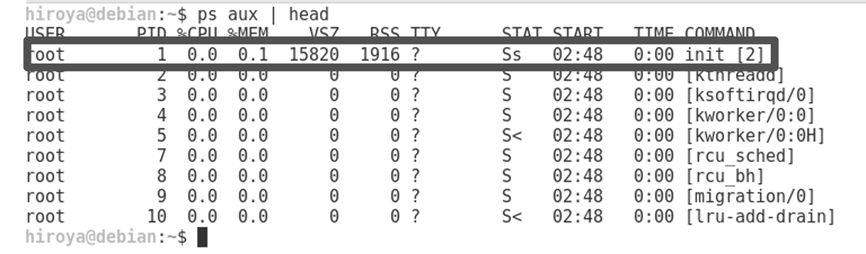
\includegraphics[keepaspectratio,width=0.5\hsize]{image201905-kansai/init01_gray.png}
 \\
  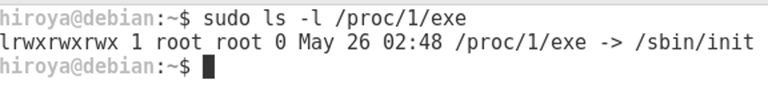
\includegraphics[keepaspectratio,width=0.5\hsize]{image201905-kansai/init02_gray.png}
 \\
  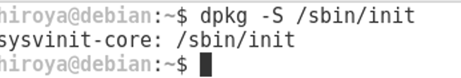
\includegraphics[keepaspectratio,width=0.3\hsize]{image201905-kansai/init03_gray.png}
 \\
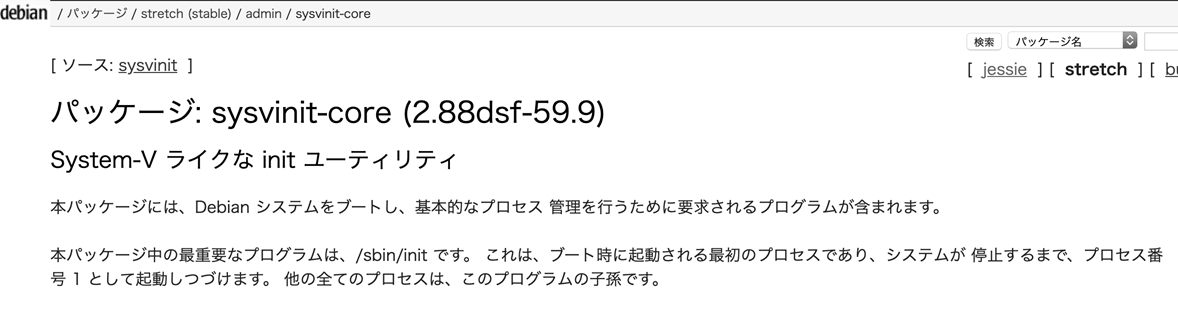
\includegraphics[keepaspectratio,width=0.7\hsize]{image201905-kansai/init04_gray.png}
\end{flushleft}

\subsection{Initプロセスを見てみる(systemd)}
\begin{flushleft}
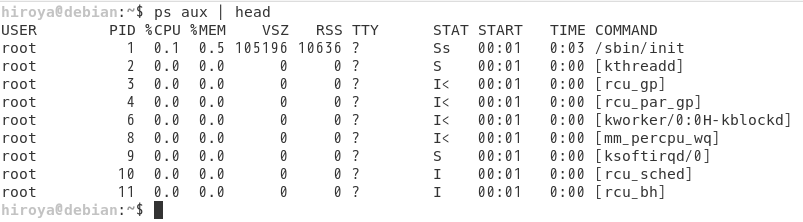
\includegraphics[keepaspectratio,width=0.6\hsize]{image201905-kansai/systemd01_gray.png}
 \\
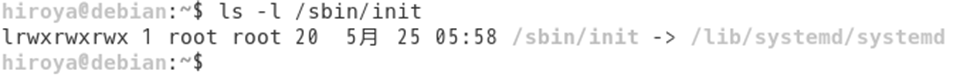
\includegraphics[keepaspectratio,width=0.6\hsize]{image201905-kansai/systemd02_gray.png}
 \\
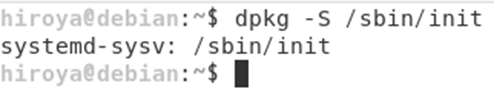
\includegraphics[keepaspectratio,width=0.4\hsize]{image201905-kansai/systemd03_gray.png}
 \\
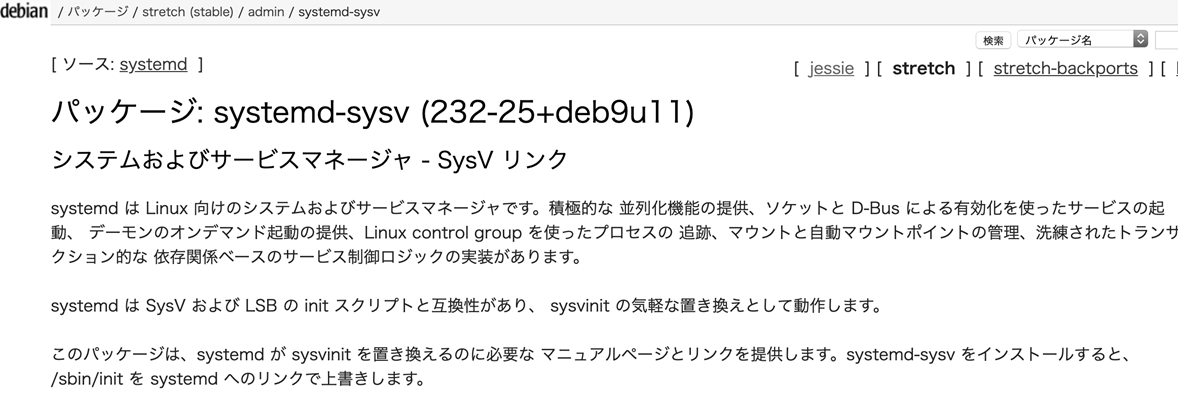
\includegraphics[keepaspectratio,width=0.7\hsize]{image201905-kansai/systemd04_gray.png}
\end{flushleft}

\subsection{systemdのメリット}
\subsubsection{これまでのinitプロセスでは以下の問題が発生していた}

\begin{itemize}
 \item シェルスクリプトを順番に実行していくので、システムの起動に時間がかかる
 \item サービスごとにcgroupsでリソース配分を調整するなどの仕組みがない
\end{itemize}

\subsubsection{systemdでは?}

\begin{itemize}
 \item プロセスの起動を出来る限り並列で行おうとするので、起動が早い
 \item Cgroupでプロセスの管理を行うので、リソース管理、生存確認などが出来る
 \item リファレンスがめっちゃ丁寧に書かれている
\end{itemize}

\subsection{sysvinitの起動プロセス}
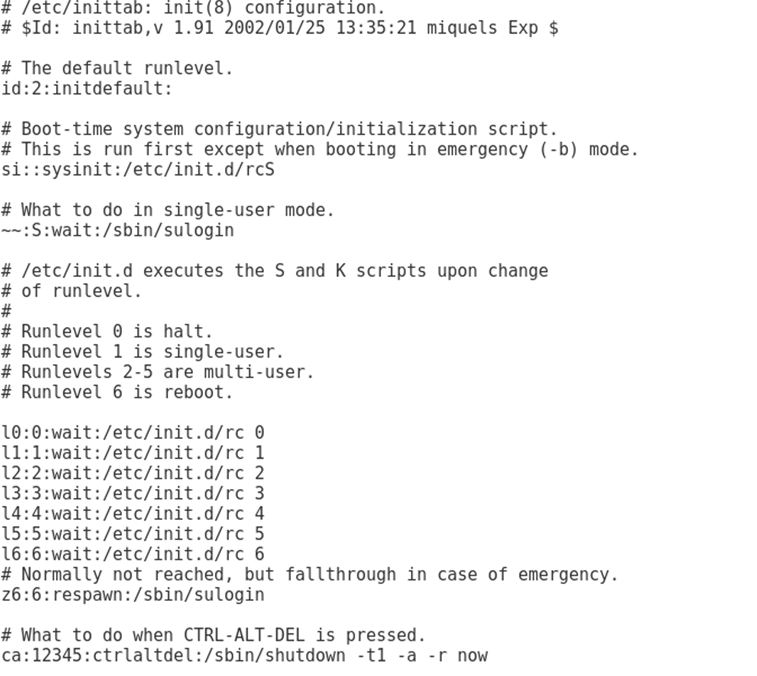
\includegraphics[keepaspectratio,width=0.5\hsize]{image201905-kansai/initboot01_gray.png}
 \\
/etc/init.d/rc
 \\
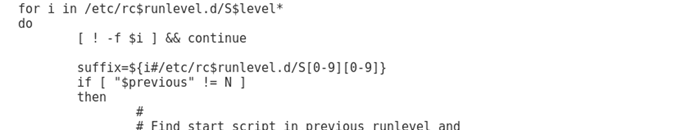
\includegraphics[keepaspectratio,width=0.7\hsize]{image201905-kansai/initboot02_gray.png}
 \\
 \\
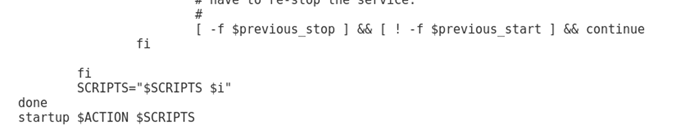
\includegraphics[keepaspectratio,width=0.7\hsize]{image201905-kansai/initboot03_gray.png}
 \\
/etc/rc*.d以下のスクリプトを
順番に実行する
 \\
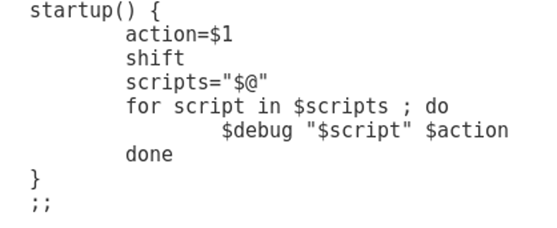
\includegraphics[keepaspectratio,width=0.4\hsize]{image201905-kansai/initboot04_gray.png}

\subsection{systemdの起動プロセス}
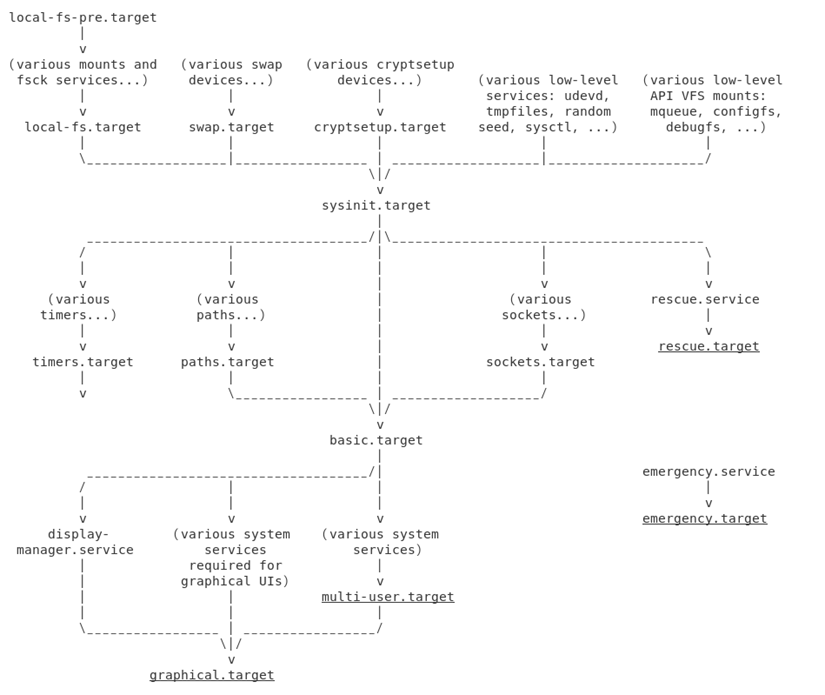
\includegraphics[keepaspectratio,width=0.7\hsize]{image201905-kansai/systemdboot01_gray.png}

\subsection{systemdのユニット}
systemdはプロセスをユニットという単位で管理する
\\
全部で11個のユニットが存在する
\begin{itemize}
 \item サービスユニット
 \item ターゲットユニット
 \item ソケットユニット
 \item …
\end{itemize}

\subsection{サービスユニット}
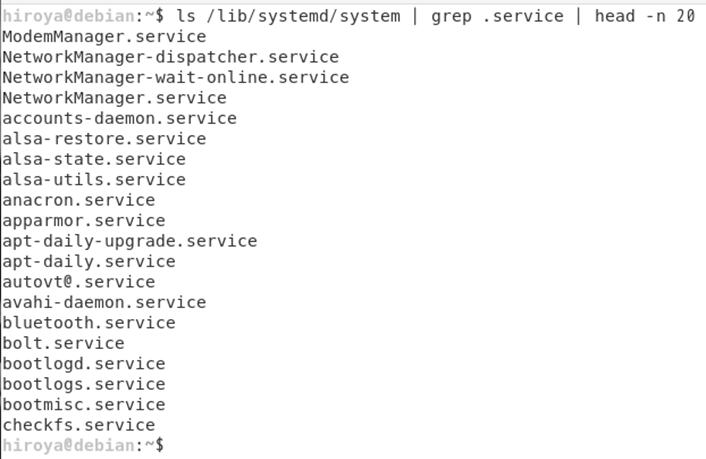
\includegraphics[keepaspectratio,width=0.5\hsize]{image201905-kansai/serviceunit01_gray.png}
\begin{itemize}
 \item プロセスを制御・管理するためのユニット
 \item .serviceで終わるユニットファイル
 \item 一般的なユースケースで使用するユニットはほとんどこれ
\end{itemize}

\subsection{ターゲットユニット}
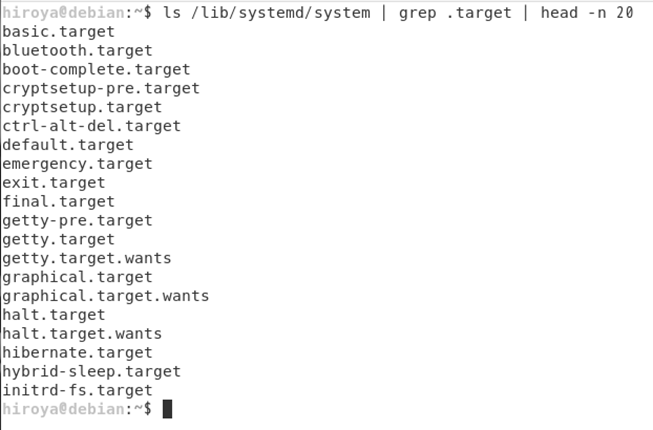
\includegraphics[keepaspectratio,width=0.5\hsize]{image201905-kansai/targetunit01_gray.png}
\begin{itemize}
 \item 複数のユニットをグルーピングするためのユニット
 \item .targetで終わるユニットファイル
 \item ユニット間の起動順序をわかりやすくするために利用される
\end{itemize}

\subsection{systemdの起動順序}
ユニットの関係性は「依存」と「順序」の2つの考え方が存在\\
依存
\begin{itemize}
 \item プロセス同士が同時起動するかどうか
 \item あくまで、同時に起動するかどうかであり、起動順序は考慮しない
\end{itemize}

順序
\begin{itemize}
 \item プロセス起動の順序関係を定義する
\end{itemize}

例えば、プロセスAがプロセスBを必要とする場合(依存)、
明示的に順序を指定しないと、プロセスAとBは同時に起動する\\

まず、default.targetから依存関係、順序関係を構築
 \\
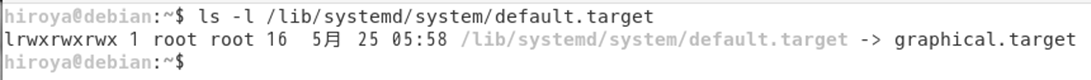
\includegraphics[keepaspectratio,width=0.7\hsize]{image201905-kansai/order01_gray.png}
 \\
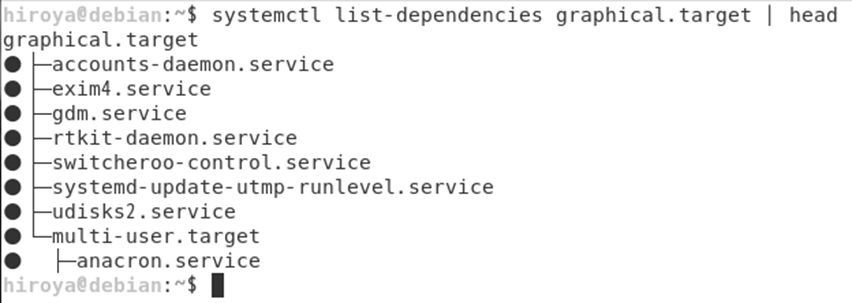
\includegraphics[keepaspectratio,width=0.7\hsize]{image201905-kansai/order02_gray.png}

\subsection{systemdではどんなプロセスが起動するの?}

sysvinitでは、/etc/rc*.d内のプロセスが起動する\\
systemdでは、以下のディレクトリのプロセスが起動対象
\begin{itemize}
 \item /etc/systemd/system(ユーザーのコンフィグ)
 \item /lib/systemd/system(インストールパッケージのコンフィグ)
\end{itemize}
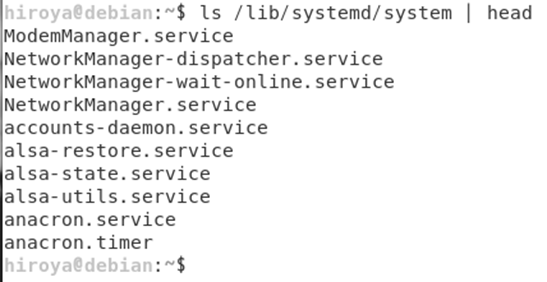
\includegraphics[keepaspectratio,width=0.5\hsize]{image201905-kansai/systemdsystem01_gray.png}

\subsection{systemctlって?}

systemdにあれこれと命令を出すことが出来るコマンド
\begin{itemize}
 \item systemctl status … unitの状態を見ることが出来る
 \item systemctl edit … drop inという起動でunitファイルを編集
 \item systemctl show/cat … unitファイルを表示
 \item systemctl enable/disable … プロセスの自動起動を制御
 \item systemctl daemon-reload … unitファイルの変更を反映
 \item systemctl start/stop/restart … プロセスの起動制御
 \item systemctl list-unit-files --type=service … サービスの一覧を表示
\end{itemize}

\subsection{実際にサービスを作ってみる(自動起動)}
sampleA.service
\begin{commandline}
[Service]
ExecStart=/bin/bash -c "date > /home/hiroya/sampleA.txt; sleep 10"

[Install]
RequiredBy=multi-user.target
\end{commandline}
現在の日時をsampleA.txtの出力するプロセス\\
multi-user.tagetの逆依存を指定
 \\
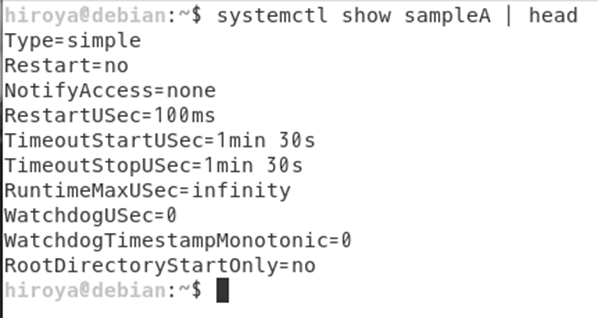
\includegraphics[keepaspectratio,width=0.5\hsize]{image201905-kansai/samplea01_gray.png}
 \\
sampleAの明示的な設定は2行だけだが、後ろでいろいろな設定が勝手に付与される

\subsection{自動起動の有効化}
 
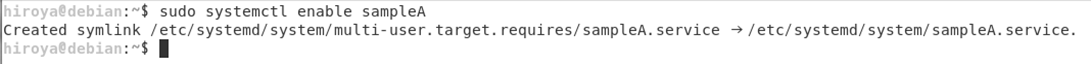
\includegraphics[keepaspectratio,width=0.8\hsize]{image201905-kansai/samplea02_gray.png}
 \\
 \\
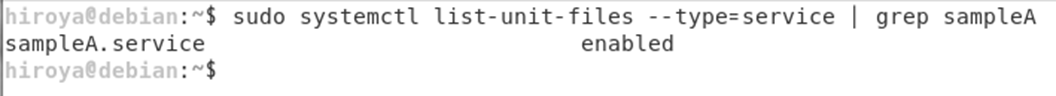
\includegraphics[keepaspectratio,width=0.8\hsize]{image201905-kansai/samplea03_gray.png}

\subsection{実際にサービスを作ってみる(依存あり)}
sampleA.service

\begin{itemize}
 \item sampleB.serviceへの依存を追加
 \item sampleAには、sampleBが必要ということ
\end{itemize}

\begin{commandline}
[Unit]
Requires=sampleB.service

[Service]
ExecStart=/bin/bash -c "date > /home/hiroya/sampleA.txt; sleep 10"

[Install]
RequiredBy=multi-user.target

\end{commandline}
sampleB.service
\begin{commandline}
[Service]
ExecStart=/bin/bash -c "date > /home/hiroya/sampleB.txt"
\end{commandline}
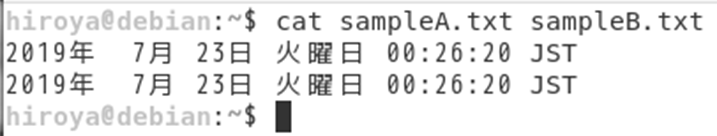
\includegraphics[keepaspectratio,width=0.5\hsize]{image201905-kansai/samplea04_gray.png}
 \\
sampleAからsampleBが呼び出されていることがわかる
また、依存のみなので、sampleAとsampleBは同時に起動している

\subsection{実際にサービスを作ってみる(順序あり)}
sampleA.service
\begin{commandline}
[Unit]
Requires=sampleB.service
Before=sampleB.service

[Service]
Type=oneshot
ExecStart=/bin/bash -c "date > /home/hiroya/sampleA.txt; sleep 10"

[Install]
RequiredBy=multi-user.target
\end{commandline}
BeforeとType=oneshotを追加することで、
sampleAの後に、sampleBを起動することが出来る
 \\
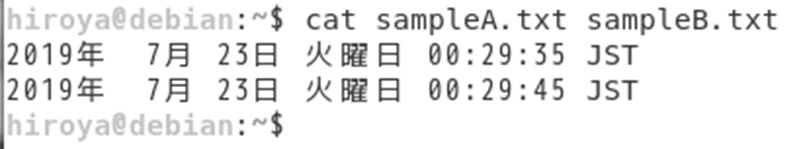
\includegraphics[keepaspectratio,width=0.5\hsize]{image201905-kansai/samplea05_gray.png}
 \\
sampleAの10秒後にsampleBが起動していることがわかる

%\subsection{おまけ}

\subsection{journalctlって?}
\begin{itemize}
 \item systemd環境では、ログの収集はjournald(system-journald)が担当
 \item journalctlはjournaldに対して命令を行う事ができるコマンド
 \item Systemdのサービスのログを表示できるので、エラーの際は便利
\end{itemize}
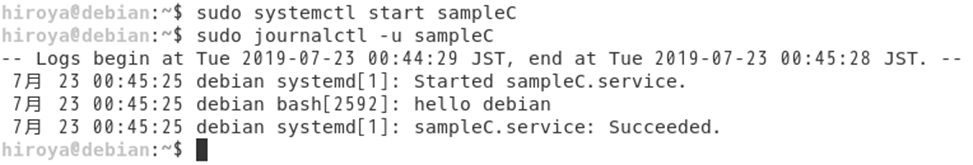
\includegraphics[keepaspectratio,width=0.7\hsize]{image201905-kansai/journalctl01_gray.png}

\subsection{graphical.targetの遷移を邪魔してみる}
sample.service
\begin{commandline}
[Unit]
Before=sysinit.target
DefaultDependencies=no
OnFailure=emergency.target

[Service]
Type=oneshot
ExecStart=/bin/false

[Install]
RequiredBy=sysinit.target
\end{commandline}
sysinit.targetが完了せず、次のターゲットに遷移せずに、
強制的にemergency.targetに遷移する\\
systemdの起動プロセス(再掲)
 \\
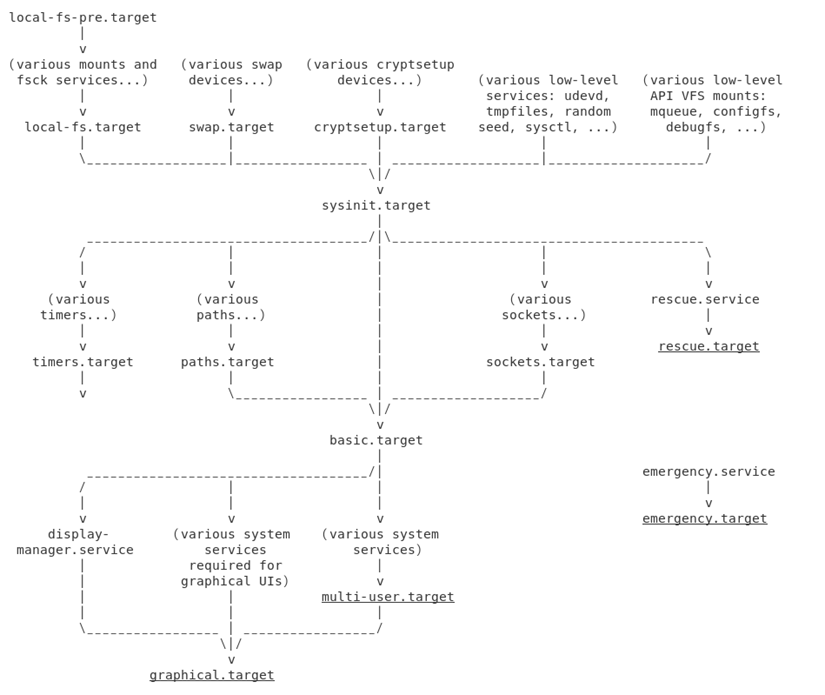
\includegraphics[keepaspectratio,width=0.7\hsize]{image201905-kansai/systemdboot01_gray.png}


sample.service
\begin{commandline}
[Unit]
Before=sysinit.target
DefaultDependencies=no
#OnFailure=emergency.target

[Service]
Type=oneshot
ExecStart=/bin/false

[Install]
RequiredBy=sysinit.target
\end{commandline}
OnFailureをコメントアウトすると、正常にOSが起動しなくなる
(プロンプト受付をしなくなる)\\
もし、sysinit.targetよりも前のサービスを作成する場合は、
OnFailureを設定しておくと安心

%ご清聴ありがとうございました

%201903 tokyo
%-------------------------------------------------------------------------------
\dancersection{systemdとsysvinitのデーモンで動作するDebianパッケージの作り方を調べてみる}{杉本 典充}
%-------------------------------------------------------------------------------

\subsection{はじめに}

デーモンプログラムをdebianパッケージ化するにはどのようにパッケージを作成すればよいのか理解していないため、調べてみました。


\subsection{Debianにおけるinitの仕組み}

一般的にUNIX/Linux系のOSにおいてカーネルが最初に呼び出す「init」というユーザランドプログラム\footnote{一般的にプロセス番号 「1」の場合が多いです。}があり、このinitが常駐プログラム(=デーモン)の起動や停止を管理します。


Debianにおけるinitシステムの解説は、Debian リファレンスの「第3章 システムの初期化」に記述があります\footnote{\url{https://www.debian.org/doc/manuals/debian-reference/ch03.ja.html}}。

Debianで採用しているinitシステムは、昔から存在する「sysvinit」、新世代の「systemd」があり\footnote{他にもOpenRCというinitもあります。}、Debian 8からはsystemdを標準のinitシステムとして採用しています\footnote{systemdが標準なのはDebian GNU/Linuxの場合です。systemdはlinuxカーネル専用のプログラムのため、kFreeBSDやHurdでは動きません。}。


Debianではsystemdとsysvinitを切り替えることができます\footnote{\url{https://wiki.debian.org/Init}}。そのためデーモンプログラムのdebianパッケージを作るときは、systemdとsysvinitのどちらの環境でもデーモンを起動できるようパッケージを作る必要があります。


\subsection{Debianにおけるinitが呼び出す起動・停止の設定ファイル}

\subsubsection{systemd: /lib/systemd/system/[package].service}

Debianのsystemdが管理するデーモンの起動・終了は、"systemctl" コマンドで行います。


systemctlコマンドで管理するデーモンの設定ファイルは、"/lib/systemd/system/[package].service" に置いています。この "[package].service" ファイルにプログラムのファイルパスや環境設定ファイル、実行するコマンドを記述します\footnote{serviceファイルの記述方法は、\url{https://www.freedesktop.org/software/systemd/man/systemd.service.html} を参照。}。


例として、nginx-fullパッケージを見てみましょう。


nginxを起動する場合は以下のコマンドを実行します。

\begin{commandline}
# systemctl start nginx
\end{commandline}

nginxを停止する場合は以下のコマンドを実行します。

\begin{commandline}
# systemctl stop nginx
\end{commandline}


上記のsystemctlコマンドを実行したとき、以下の"nginx.service"に従ってnginxの起動・終了をsystemdが行っています。


\begin{commandline}
$ cat /lib/systemd/system/nginx.service | grep -v "\#"

[Unit]
Description=A high performance web server and a reverse proxy server
Documentation=man:nginx(8)
After=network.target nss-lookup.target

[Service]
Type=forking
PIDFile=/run/nginx.pid
ExecStartPre=/usr/sbin/nginx -t -q -g 'daemon on; master_process on;'
ExecStart=/usr/sbin/nginx -g 'daemon on; master_process on;'
ExecReload=/usr/sbin/nginx -g 'daemon on; master_process on;' -s reload
ExecStop=-/sbin/start-stop-daemon --quiet --stop --retry QUIT/5 --pidfile /run/nginx.pid
TimeoutStopSec=5
KillMode=mixed

[Install]
WantedBy=multi-user.target  
\end{commandline}


\subsubsection{sysvinit: /etc/init.d/[package]}

Debianのsysvinitが管理するデーモンの起動・終了は、"service"コマンドで行います\footnote{Debian GNU/Linux 8 以降ではsystemdがデフォルトのため \url{https://wiki.debian.org/Init} の手順を行うとsysvinitに変更できます。}。


serviceコマンドで管理するデーモンの設定ファイルは、"/etc/init.d/[package]"に置いています。この"[package]"ファイルはシェルスクリプトであり、プログラムのファイルパスや環境設定ファイル、実行するコマンドを記述します。


serviceコマンドから呼び出すスクリプトを作成するにあたり、以下のヘルパースクリプトがあります。

\begin{itemize}
  \item /lib/init/vars.sh
  \item /lib/lsb/init-functions
  \item /sbin/start-stop-daemon
\end{itemize}


例として、nginx-fullパッケージを見てみましょう。


nginxを起動する場合は以下のコマンドを実行します(systemctlの場合とコマンドの順番が違います)。

\begin{commandline}
# service nginx start
\end{commandline}

nginxを停止する場合は以下のコマンドを実行します。

\begin{commandline}
# service nginx stop
\end{commandline}


上記のserviceコマンドを実行したとき、nginxの起動・終了を "/etc/init.d/nginx" が行っています。

※長いため一部省略しています。

\begin{commandline}
$ cat /etc/init.d/nginx

#!/bin/sh

### BEGIN INIT INFO
# Provides:       nginx
# Required-Start:    $local_fs $remote_fs $network $syslog $named
# Required-Stop:     $local_fs $remote_fs $network $syslog $named
# Default-Start:     2 3 4 5
# Default-Stop:      0 1 6
# Short-Description: starts the nginx web server
# Description:       starts nginx using start-stop-daemon
### END INIT INFO

PATH=/usr/local/sbin:/usr/local/bin:/sbin:/bin:/usr/sbin:/usr/bin
DAEMON=/usr/sbin/nginx
NAME=nginx
DESC=nginx

# Include nginx defaults if available
if [ -r /etc/default/nginx ]; then
        . /etc/default/nginx
fi

STOP_SCHEDULE=''${STOP_SCHEDULE:-QUIT/5/TERM/5/KILL/5}''

test -x $DAEMON || exit 0

. /lib/init/vars.sh
. /lib/lsb/init-functions

# Try to extract nginx pidfile
PID=$(cat /etc/nginx/nginx.conf | grep -Ev '^\s*#' | awk 'BEGIN { RS=''[;{}]'' } { if ($1 == ``pid'') print $2 }' | head -n1)
if [ -z ``$PID'' ]; then
    PID=/run/nginx.pid
fi

if [ -n ``$ULIMIT'' ]; then
    # Set ulimit if it is set in /etc/default/nginx
    ulimit $ULIMIT
fi

start_nginx() {
    # Start the daemon/service
    #
    # Returns:
    #   0 if daemon has been started
    #   1 if daemon was already running
    #   2 if daemon could not be started
    start-stop-daemon --start --quiet --pidfile $PID --exec $DAEMON --test > /dev/null \
        || return 1
    start-stop-daemon --start --quiet --pidfile $PID --exec $DAEMON -- \
        $DAEMON_OPTS 2>/dev/null \
        || return 2
}

  (snip)

stop_nginx() {
    # Stops the daemon/service
    #
    # Return
    #   0 if daemon has been stopped
    #   1 if daemon was already stopped
    #   2 if daemon could not be stopped
    #   other if a failure occurred
    start-stop-daemon --stop --quiet --retry=$STOP_SCHEDULE --pidfile $PID --name $NAME
    RETVAL=''$?''
    sleep 1
    return ``$RETVAL''
}

(snip)

case ``$1'' in
    start)
        log_daemon_msg ``Starting $DESC'' ``$NAME''
        start_nginx
        case ``$?'' in
            0|1) log_end_msg 0 ;;
            2)   log_end_msg 1 ;;
        esac
        ;;
    stop)
        log_daemon_msg ``Stopping $DESC'' ``$NAME''
        stop_nginx
        case ``$?'' in
            0|1) log_end_msg 0 ;;
            2)   log_end_msg 1 ;;
        esac
        ;;

(snip)

    *)
        echo ``Usage: $NAME {start|stop|restart|reload|force-reload|status|configtest|rotate|upgrade}'' >&2
        exit 3
        ;;
esac
\end{commandline}


\subsection{init設定を行うdebianパッケージ作成方法}

\subsubsection{前提}

Debian GNU/Linux 9 (stretch) の環境を前提とします。


debianパッケージを作成するツールは、ほとんどのパッケージでdebhelperが使われています\footnote{\url{https://www.debian.org/doc/manuals/packaging-tutorial/packaging-tutorial.ja.pdf} の2019年3月4日の資料において debhelperの採用率は98\%との数字があります。} 。今回は、debhelperを使ってパッケージ作成を行うことを前提として説明します。


debianパッケージを作成するにあたり、基本的な事項を知るドキュメントは以下になりますので読んでみてください。

\begin{itemize}
\item \url{https://wiki.debian.org/ja/Packaging}
\item packaging-tutorialパッケージのPDFファイル \\/usr/share/doc/packaging-tutorial/packaging-tutorial.ja.pdf\footnote{web版はこちら。 \url{https://www.debian.org/doc/manuals/packaging-tutorial/packaging-tutorial.ja.pdf}}
\item Debian 新メンテナーガイド \\\url{https://www.debian.org/doc/manuals/maint-guide/index.ja.html}
\item Debian Policy Manual \\\url{https://www.debian.org/doc/debian-policy/}
\end{itemize}  


debhelperでdebianパッケージの作成を行う場合は以下のパッケージをインストールしておくとよいでしょう\footnote{昔はsystemdに対応する場合にはdh-systemdパッケージが必要でしたが、stretchではdebhelperに統合されているためインストール不要です。}。


\begin{commandline}
# apt-get update
# apt-get install build-essential dpkg-dev devscripts debhelper dh-make quilt
\end{commandline}


\subsubsection{systemdに対応する設定}

以下のwebページに解説ドキュメントがありますので、これを解説していきます。

\begin{itemize}
\item \url{https://wiki.debian.org/Teams/pkg-systemd/Packaging}
\end{itemize}


systemdの設定を行うには通常のパッケージ作成作業のほか、以下を追加で作業する必要があります。

\begin{itemize}
\item debian/rulesの修正
\item debian/controlの修正
\item \bf{"debian/package.service"} の作成
\end{itemize}


\subsubsubsection{debian/rulesの修正}

debian/rulesファイルは、dh\_makeコマンドを実行したときにひな形ファイルが作成されます。


systemdで管理するデーモンの場合は、以下のように "--with systemd" の定義を追加します。この "--with" オプションは debhelper の addon の処理を実行するように指定するものです\footnote{man dh(1) を参照。}。

\begin{commandline}
%:
    dh $@ --with systemd
\end{commandline}


この "--with systemd" の addon 指定がある場合は debian パッケージのビルド処理で "dh\_systemd\_enable"、 "dh\_systemd\_start" を実行するようになります。


"dh\_systemd\_enable" は、"\# systemctl \{enable/disable\} package" を実行するよう指定するもので、次回のOS起動時に自動で package のデーモンを起動するか指定できます。


"dh\_systemd\_start" は、"\# systemctl \{start/stop/restart\} package" を実行するよう指定するコマンドで、パッケージのインストール処理でデーモンを起動するか、再起動するかなどを指定できます。


\subsubsubsection{debian/controlの修正}

"debian/control"ファイルは、dh\_makeコマンドを実行したときにひな形ファイルが作成されます。


"debian/control" ファイルを書く上で、debhelperの互換性レベルを記述する"debian/compat" ファイルがあります。この"debian/compat"ファイルの中身が"10"以上であれば "debian/control" ファイルを次のように書きます。

\begin{commandline}
Build-Depends: debhelper (>= 9.20160709)
\end{commandline}

もし、"debian/compat" の中身が "10" 未満であれば systemd 向けの処理は別途 dh-systemd パッケージが必要なため\footnote{Debian 8 jessie 向けのパッケージを作成する場合が該当します。}、次のように書きます。

\begin{commandline}
Build-Depends: debhelper (>= 9.20150101), dh-systemd (>= 1.5)
\end{commandline}


\subsubsubsection{debian/package.service の作成}


"package.service" ファイルは、dh\_makeコマンドを実行したときにひな形ファイルが作成されません。

そのため、他のパッケージの "package.service" ファイルを参考にしつつ、serviceファイルのマニュアルをみて作成してください\footnote{\url{https://www.freedesktop.org/software/systemd/man/systemd.service.html}}

"package.service" ファイルを作成しておくと、debian パッケージのビルド処理中の "dh\_installinit" の処理で "package.service" ファイルを "/lib/systemd/system" 配下へインストールするよう処理します。


\subsubsection{sysvinitに対応する設定}


sysvinitの設定を行うには、通常のパッケージ作成作業のほか、以下を追加で作業する必要があります。

\begin{itemize}
\item \bf{"debian/package.init"} の作成
\end{itemize}


\subsubsubsection{debian/package.init の作成}


"packages.init" ファイルは、dh\_makeコマンドを実行したときにひな形ファイルが作成されません\footnote{過去にはdh\_makeコマンドで"debian/init.d.ex" というひな形ファイルが作成されたのですが、Debian 8におけるsystemdへの移行の過程で作成されなくなりました。}。


他のパッケージのinitファイルを参考にするか、古いバージョンのdebhelperに含まれる"init.d.ex" ファイルを取得して作成してください\footnote{\url{https://sources.debian.org/data/main/d/dh-make/1.20140617/lib/debian/init.d.ex}}。


"package.init" ファイルを作成しておくと、debianパッケージのビルド処理中の "dh\_installinit"の処理で "package.init" ファイルを "/etc/init.d" 配下へインストールするよう処理します。


\subsection{まとめ}

Debianにおけるinitの説明とデーモンの起動・終了を行うdebianパッケージをdebhelperでどう作るか説明しました。debian/[package].service ファイル、debian/[package].init ファイルの存在を覚えておくとよいと思います。


debhelperを使ったdebianパッケージのビルドでは  dh\_installinit の処理で systemd/sysvinit の設定ファイルをパッケージに配置しています。


また、1つのソースパッケージから複数のバイナリパッケージを作る場合にファイル名の命名規則が異なるなど違いも出てきます。それらについては他のパッケージを参考にして覚えていくとよいと思います。


\subsection{参考文献}

\begin{itemize}
\item 「Teams pkg-systemd Packaging」 \url{https://wiki.debian.org/Teams/pkg-systemd/Packaging}
\item mkouhei (2014) 「How to create a Debian package of support to sysvinit, upstart, systemd」 \url{https://d.palmtb.net/2014/01/30/how_to_create_a_debian_package_of_support_to_sysvinit__upstart__systemd.html}
\item @henrich (2016) 「dh-systemdはdebhelper 9.20160709で統合された」 \url{https://qiita.com/henrich/items/e1651e3284c6b3d0d39e}
\end{itemize}

%201904 debianmeetingresume201904-knok.tex
\dancersection{grml-debootstrapを用いたUSB起動メモリの作成}{野首 貴嗣}

(発表資料から編集者が適当に変換したので見にくいところはご容赦ください。)

\subsection{自己紹介}

  \begin{itemize}
  \item NOKUBI Takatsugu (野首 貴嗣)
  \item knok@debian.org / knok@daionet.gr.jp
  \item Twitter: @knok
  \item Debian developer since 2002
  \item bo 時代からのマシンを運用し続けている
  \end{itemize}


\subsection{目次}

  \begin{itemize}
  \item USBメモリを使う動機
  \item grml-debootstrap概要
  \item セットアップ準備
  \item 設定
  \item ブートローダーの設定
  \end{itemize}


\subsection{USBメモリを使う動機}

  \begin{itemize}
  \item 内臓ストレージに影響なし
  \item USBメモリ以外の手法
    \begin{itemize}
    \item chroot環境(debootstrap)
      \begin{itemize}
      \item daemon類の扱いが面倒
      \end{itemize}
    \item コンテナ(LXC/LXD/Docker等)
    \item 完全仮想環境(VirtualBox, KVM等)
      \begin{itemize}
      \item 物理デバイスを扱いたい時大変
      \end{itemize}
    \end{itemize}
  \end{itemize}


  \begin{itemize}
  \item 物理マシンの環境を汚さない
    \begin{itemize}
    \item 大抵はライセンスされたproprietary OSが入っている
    \item リカバリー領域、診断ツールなど
    \end{itemize}
  \item 一つのメディアを複数のデバイスで使える
  \item 複数のデバイスを用意すれば異なる環境を用意できる
  \item 物理デバイスすべてを扱える
    \begin{itemize}
    \item 仮想環境と比較して
    \end{itemize}
  \item NASの起動デバイスとして(Microserver)
  \end{itemize}

\subsection{grml-debootstrap}


GRML Live Linuxの一部
\begin{itemize}
  \item \url{http://grml.org/}
    \begin{itemize}
    \item システム管理者向けLive Linux環境
    \item FAIに対応
    \end{itemize}
  \item パッケージメンテナンス: Grml Team
  \item 関連ツール: grml-rescueboot, grml2usb
  \item ソースコード: \url{https://github.com/grml/grml-debootstrap}
\end{itemize}



\subsection{セットアップ準備}

USBメモリの選定
  \begin{itemize}
  \item 用途と容量
    \begin{itemize}
    \item デスクトップ用途なら32GBもあれば十分
    \item ストレージを使わないサーバー用途なら16GB程度で十分
    \end{itemize}
  \item 速度
  \item 耐久性
    \begin{itemize}
    \item 安物はヘビーなアクセスが蓄積するとすぐ壊れる
    \end{itemize}
  \end{itemize}

  \begin{itemize}
  \item EFIに対応する
    \begin{itemize}
    \item EFI領域を分ける必要あり
    \item GPTを使う
    \item オプション: MBRにも対応するなら2048セクタ目からパーティションを開始する
    \end{itemize}
  \item 方針: スワップパーティションは作らない
  \item rootファイルシステムの選択
    \begin{itemize}
    \item ext4
    \item f2fs - 最新のgrubでしか対応していない点に注意
    \end{itemize}
  \end{itemize}

\subsection{設定}

  \begin{commandline}
$ sudo gdisk /dev/sda
GPT fdisk (gdisk) version 1.0.1
Command (? for help): n
Partition number (1-128, default 1): 
First sector (34-31358942, default = 2048) or {+-}size{KMGTP}: 
Last sector (2048-31358942, default = 31358942) or {+-}size{KMGTP}: +256M
Current type is 'Linux filesystem'
Hex code or GUID (L to show codes, Enter = 8300): ef00
Changed type of partition to 'EFI System'

Command (? for help): n
Partition number (2-128, default 2): 
First sector (34-31358942, default = 526336) or {+-}size{KMGTP}: 
Last sector (526336-31358942, default = 31358942) or {+-}size{KMGTP}: 
Current type is 'Linux filesystem'
Hex code or GUID (L to show codes, Enter = 8300): 
Changed type of partition to 'Linux filesystem'

Command (? for help): w

Final checks complete. About to write GPT data. THIS WILL OVERWRITE EXISTING
PARTITIONS!!

Do you want to proceed? (Y/N): y
OK; writing new GUID partition table (GPT) to /dev/sda.
The operation has completed successfully.
\end{commandline}


\subsection{インストール}

  \begin{commandline}
$ sudo mkfs.vfat -F32 /dev/sda1         
mkfs.fat 4.1 (2017-01-24)
sudo mkfs -t f2fs /dev/sda2

        F2FS-tools: mkfs.f2fs Ver: 1.7.0 (2016-07-28)

Info: Debug level = 0
Info: Label = 
Info: Trim is enabled
Info: Segments per section = 1
Info: Sections per zone = 1
Info: sector size = 512
Info: total sectors = 30832607 (15054 MB)
Info: zone aligned segment0 blkaddr: 256
Info: format version with
  "Linux version 4.18.0-0.bpo.1-amd64 (debian-kernel@lists.debian.org) (gcc version 6.3.0 20170516 (Debian 6.3.0-18+deb9u1)) 
  #1 SMP Debian 4.18.6-1~bpo9+1 (2018-09-13)"
Info: Discarding device
Info: This device doesn't support BLKSECDISCARD
Info: This device doesn't support BLKDISCARD
Info: Overprovision ratio = 1.640%
Info: Overprovision segments = 249 (GC reserved = 129)
Info: format successful
  \end{commandline}

--efiオプションはEFI環境で起動していないと動作しない点に注意
  \begin{commandline}
$ sudo grml-debootstrap -m http://deb.debian.org/debian -r stretch -t /dev/sda2 --efi /dev/sda1 \
  --grub /dev/sda --arch amd64 --filesystem ext4 --password toor
 * EFI support detected.
 * grml-debootstrap [0.78] - Please recheck configuration before execution:

   Target:          /dev/sda2
   Install grub:    /dev/sda
   Install efi:     /dev/sda1
   Using release:   stretch
   Using hostname:  xps13
   Using mirror:    http://deb.debian.org/debian
   Using arch:      amd64
   Config files:    /etc/debootstrap

   Important! Continuing will delete all data from /dev/sda2!

 * Is this ok for you? [y/N] y
 * EFI partition /dev/sda1 seems to have a FAT filesystem, not modifying.
 * Running mkfs.f2fs  on /dev/sda2

        F2FS-tools: mkfs.f2fs Ver: 1.7.0 (2016-07-28)

Info: Debug level = 0
Info: Label =
Info: Trim is enabled
Info: Segments per section = 1
Info: Sections per zone = 1
Info: sector size = 512
Info: total sectors = 30832607 (15054 MB)
Info: zone aligned segment0 blkaddr: 256
Info: format version with
  "Linux version 4.18.0-0.bpo.1-amd64 (debian-kernel@lists.debian.org) (gcc version 6.3.0 20170516 (Debian 6.3.0-18+deb9u1)) 
  #1 SMP Debian 4.18.6-1~bpo9+1 (2018-09-13)"
Info: Discarding device
Info: This device doesn't support BLKSECDISCARD
Info: This device doesn't support BLKDISCARD
Info: Overprovision ratio = 1.640%
Info: Overprovision segments = 249 (GC reserved = 129)
Info: format successful
blockdev: ioctl error on BLKRRPART: Device or resource busy
/usr/sbin/grml-debootstrap: line 1119: filesystem: command not found
 * Mounting /dev/sda2 to /mnt/debootstrap.4583
 * Running debootstrap  for release stretch (amd64) using http://deb.debian.org/debian
 * Executing: debootstrap --arch amd64   stretch /mnt/debootstrap.4583 http://deb.debian.org/debian
I: Retrieving InRelease
I: Retrieving Release
I: Retrieving Release.gpg
I: Checking Release signature
I: Valid Release signature (key id 067E3C456BAE240ACEE88F6FEF0F382A1A7B6500)
I: Retrieving Packages
I: Validating Packages
I: Resolving dependencies of required packages...
I: Resolving dependencies of base packages...


Finished chroot installation, exiting.
 * Removing chroot-script again
 * Unmount /mnt/debootstrap.4583
 * Removing /var/cache/grml-debootstrap/variables_sda2
 * Removing /var/cache/grml-debootstrap/stages_sda2
 * Finished execution of grml-debootstrap. Enjoy your Debian system.
  \end{commandline}


EFIパーティションの/EFI/BOOT以下にBOOTX64.EFIという名称でファイルを配置
\begin{commandline}
# mount /dev/sda1 /mnt
# cd /mnt/EFI
# mkdir BOOT
# cp /boot/efi/EFI/debian/grubx64.efi BOOT/BOOTX64.EFI
# umount /mnt
\end{commandline}
同様にgrub-efi-ia32を用いてBOOT/BOOTx32.EFIを用意すれば32bit UEFI対応もできる
\\
MBRに書き込めばEFI/MBR両対応も可能

\subsection{動作確認}

  \begin{itemize}
  \item diskグループに追加
    \begin{itemize}
    \item sudo adduser user disk
    \item ログインし直す
    \end{itemize}
  \item Raw diskに対応するvmdkの作成
    \begin{commandline}
      $ vboxmanage internalcommands createrawvmdk -filename \
      ~/usb.vmdk -rawdisk /dev/sda
    \end{commandline}
  \item VirtualBoxで仮想マシンを作成
    \begin{itemize}
    \item ストレージに先程作成したusb.vmdkを指定
    \item UEFIを有効化
    \end{itemize}
  \item 起動
  \end{itemize}

  \begin{itemize}
  \item 起動ストレージ
    \begin{itemize}
    \item fstab, grub.cfgにUUIDで記述
    \end{itemize}
  \item Network
    \begin{itemize}
    \item if addrでインターフェース名を確認してdhclient
    \end{itemize}
  \item Timezone
    \begin{itemize}
    \item dpkg-reconfigure tzdata
    \end{itemize}
  \item Hardware Clock
    \begin{itemize}
    \item /etc/adjtimeの末尾修正
    \item LOCALでRTCをローカル扱いに
    \end{itemize}
  \item Keymap
    \begin{itemize}
    \item dpkg-reconfigure keyboard-configuration
    \item \url{https://wiki.debian.org/Keyboard}
    \item お好みで XKBOPTIONS="ctrl:swapcaps"
    \end{itemize}
  \end{itemize}

  \begin{itemize}
  \item grml-debootstrapを紹介
    \begin{itemize}
    \item インストーラを使わずストレージにDebian環境を構築
    \end{itemize}
  \item USBメモリを使う動機
    \begin{itemize}
    \item 複数のデバイスで同じ環境を利用できる
    \item メディアを分けることで異なる用途に使える
    \item 起動マシンの環境を汚さない
    \end{itemize}
  \item UEFI環境向けにデフォルトのブートローダーを配置
  \item VirtualBoxを動作テストに使える
    \begin{itemize}
    \item 細かい調整、パッケージの変更などもできる
    \end{itemize}
  \end{itemize}

\subsection{参考文献}


参考文献
  \begin{itemize}
  \item BIOS, UEFI両方で起動可能なdebianインストールUSBメディアを作る \url{http://pman0214.github.io/blog/debian-install-bios-efi.html}
  \item 32bit UEFI 搭載の2-in-1 PCにubuntu14.04をインストールした記録 \url{https://qiita.com/shirotamago/items/a4b0c8863a492abe50ad}
   \item Boot your USB Drive in VirtualBox \url{http://agnipulse.com/2009/07/boot-your-usb-drive-in-virtualbox/}
  \end{itemize}

  F2FSはどうか?
  \begin{itemize}
  \item 寿命は伸びるかも?(未検証)
    \begin{itemize}
    \item USBメモリでTRIMは発行できるか
    \item デバイス依存, hdparm -Iで確認
    \end{itemize}
  \item stretchのgrub2はf2fsをサポートしていない
    \begin{itemize}
      \item /boot を別に作ることで対応可能
    \end{itemize}
  \item パフォーマンス
    \begin{itemize}
    \item F2FS Benchmarks From USB Flash Storage (Phoronix) \url{https://www.phoronix.com/scan.php?page=article&item=linux_f2fs_usb3&num=1}
    \item 一長一短?
    \end{itemize}
  \end{itemize}

\dancersection{\mbox{Rustで書いたツールの}\mbox{debianパッケージングに}\mbox{挑戦してみた話(仮)}}{小林 克希}

\subsection{はじめに}

今回の内容ですが、最近個人的に触りだしたRustというプログラミング言語について、
そもそもどういう言語なんだというご紹介(といっても、私も勉強中の身ですが)と、
Rustで書いたツールのdebを作ってみる、というところまでを目標としています。

\subsection{Rustとは}

Rustとは、MozillaがブラウザエンジンServoのために開発したシステムプログラミング言語です。
2018年のスタックオーバーフローの調査%
\footnote{\url{https://insights.stackoverflow.com/survey/2018}}%
で愛されている言語ランキング1位になるなど、
最近では結構メジャーになっていている感じの言語です。
特徴としては、安全性・並行性について考えられて設計されている点で、
かつ、みんな大好き(?)静的型付け言語です。

なお、Rustプログラマーの事をrustacean(ラストシアン)というようです。
これは、``Crustacean(甲殻類)`` から来ているらしく、
そのせいか、オライリー本の表紙はオオヒロバオウギガニというカニですし、
非公式マスコットもかわいらしいカニ(名前はFerris%
\footnote{\url{http://rustacean.net/}}%
)になってます。

\subsubsection{Rustのツールチェーンをインストール}

ではさっそくRustのツールチェーンをインストールしてみましょう。
さて、もちろんRustのツールチェーンのdebianパッケージはありますし、
ローカルマシンにインストールせずにブラウザで色々試せるサイト%
\footnote{\url{https://play.rust-lang.org/}}
もあるのですが、Rustは2018年の年末に2018 Edition%
\footnote{\url{https://blog.rust-lang.org/2018/12/06/Rust-1.31-and-rust-2018.html}}%
という大きめな改版があったので、
ひとまずRust公式の手段でツールチェーンをインストールしましょう。
例によって例のごとく、皆様の大事なホームディレクトリに色々と入れてしまいますが、
バージョンアップの頻度はそれなりにあるので、Rustの最新を追っていくなら、
無理せずに公式のツールチェーンを入れてしまった方が無難かと思います。

Rustのツールチェーンですが、以前はそうでもなかったみたいですが、最近ではrustup%
\footnote{\url{https://rustup.rs/}}%
というインストーラーを使うのが公式手順のようです。
いかにも最近のツールっぽいですが、以下のようにcurlコマンドを叩いてインストールします。

\begin{commandline}
% curl https://sh.rustup.rs -sSf | sh
\end{commandline}

rustupを使うと、バイナリは \verb|~/.cargo| 以下にインストールされます。
パスを通したい場合、 \verb|~/.cargo/env| というファイルがあるので、
そちらを \texttt{source} してあげるとよろしいかと思います。
ひとまず、 \texttt{cargo} というコマンドが使えるようになっていたら大丈夫です。
なお、「どうしてもdebで」という方は \texttt{cargo} パッケージをインストールしてください。
その際、\texttt{rustc}のバージョンが2018 Editionである1.31以降である事が望ましいです。

\subsubsection{Hello Worldしてみる}

では、cargoが使えるようになったところで、Hello Worldしてみましょう。
Rustのプロジェクトは、 \verb|cargo new| で作成することができます。
昔は\verb|--bin|をつけないとライブラリ用のプロジェクトになってましたが、
最近のcargoであればデフォルトがバイナリ用のプロジェクトになります。
それでは実行してみましょう。

\begin{commandline}
% cargo new hello
     Created binary (application) `hello` package
% tree
.
├── Cargo.toml
└── src
    └── main.rs

1 directory, 2 files
\end{commandline}

実行すると、こんな感じにCargo.tomlというファイルと、
main.rsというソースファイルが作成されます。
そう、Rustのソースファイルの拡張子は.rsです。
そのため、Rustのプロジェクトのウェブサイトは、.rsドメインで作られてる事がおおいです。
ちなみに、.rsはセルビアのドメインです。

実は、この時点でHello Worldの半分が完了しています。
src/main.rsの中身を見てみましょう。

\begin{commandline}
fn main() {
    println!("Hello, world!");
}
\end{commandline}

なんと、既にHello Worldのコードが生成されています。
なお、詳細は省きますが、 \verb|println!()| は関数に見えますが、
ビックリマークが付いている物は、Rustではマクロであったりします。
まぁ、深く付き会う前は、特に気にしなくて良いかと思います。
ビルドして実行するには \verb|cargo run| すればOKです。

\begin{commandline}
% cargo run
   Compiling hello v0.1.0 (/path/to/hello)
    Finished dev [unoptimized + debuginfo] target(s) in 0.31s
     Running `target/debug/hello`
Hello, world!
\end{commandline}

\subsection{Rustの構文等の紹介}

それでは、ここからは簡単にRustの構文等の紹介をしていきたいと思います。
なお、私も勉強中の身ですので、微妙に嘘を書いていたらすいません。
正確な事は、The Book%
\footnote{\url{https://doc.rust-lang.org/book/}}%
と呼ばれる気合の入ったドキュメントがありますのでそちらを参考にしていただけたらと思います。

なお、Rustは比較的学習が難しいとか言われてますが、
なんで難しいのかについて、個人的にはオライリーのRust本で引用されてるQuoraに書かれたコメント%
\footnote{\url{https://www.quora.com/What-do-C-C++-systems-programmers-think-of-Rust/answer/Mitchell-Nordine}}%
がしっくり来たので引用しておきます。
\begin{quotation}
I've found that Rust has forced me to learn many of the things that I was slowly learning as
``good practise'' in C/C++ before I could even compile my code.
\end{quotation}
私は最近会社の仕事の関係でC++の勉強もするハメになってるのですが、まさに上記と同じ感想です。
なにか、C++がこなれて来て、C++11あたりでようやく良い感じになった機能だけを取り入れていったのが
Rustなんじゃないかなぁと。

\subsubsection{変数宣言}

変数の宣言は\texttt{let}キーワードを使います。
型は、最近の言語っぽくコロンの後に書きますが、型が推論できるなら省略可能です。
また、シャドーイングすることも可能で、指定がなければimmutableな変数になるので、
mutableな変数を作る場合は\texttt{mut}キーワードを使います。
具体的な例を以下に示します。

\begin{commandline}
fn main() {
    let x = 1;
    println!("x = {}", x);
    let x = 1.25;
    println!("x = {}", x);
    x = 1;   // エラーになる(そもそもimmutableだけど): expected floating-point number, found integer
    x = 1.5; // エラーになる: cannot assign twice to immutable variable

    let mut y: u32 = 1;
    y -= 1;
    y -= 1;
    println!("y = {}", y);
}
\end{commandline}

例の2つ目の\verb|y -= 1;|ですが、デバッグビルドだとオーバーフローを検知して実行時にパニックを起こします。
リリースビルド(\verb|--release|オプション付きで\texttt{cargo}を実行)だと
パニックは発生しませんが、もちろんおかしな値が表示されます。

なお、基本的な型は以下のようなものがあります。

\begin{quote}
\begin{description}
 \item[整数]
	    \textbf{符号無し:} \texttt{u8}, \texttt{u16}, \texttt{u32}, \texttt{u64}, \texttt{usize}\\
	    \textbf{符号付き:} \texttt{i8}, \texttt{i16}, \texttt{i32}, \texttt{i64}, \texttt{isize}
 \item[浮動小数点] \textbf{単精度:} \texttt{f32}、\textbf{倍精度:} \texttt{f64}
 \item[ブール] \texttt{bool}
 \item[文字] \texttt{char}  (Unicodeの1文字)
 \item[文字列] \texttt{String}
	    \begin{itemize}
	     \item ただし、文字列リテラルの \texttt{str} があってとてもややこしい
	    \end{itemize}
 \item[配列] \texttt{[T; N]} (\texttt{T}: 型,  \texttt{N}: 要素数)
 \item[ベクター] \texttt{Vec<T>} (\texttt{T}: 型)
 \item[スライス] \texttt{\&[T]} (\texttt{T}: 型)
\end{description}
\end{quote}

\texttt{String}と\texttt{str}が少々ややこしいですが、
イメージとしてはC++の\texttt{std::string}と\texttt{char}の関係に近いような感じです。
\texttt{String}の方は可変長で、メモリ上のイメージを図にすると図\ref{fig:str-string}のような感じです。
\texttt{\&}がついてる\texttt{str}は、この後述する参照になってます。
ひとまず、以下がちょっとしたサンプルコードです。

\begin{figure}[htbp]
 \begin{center}
  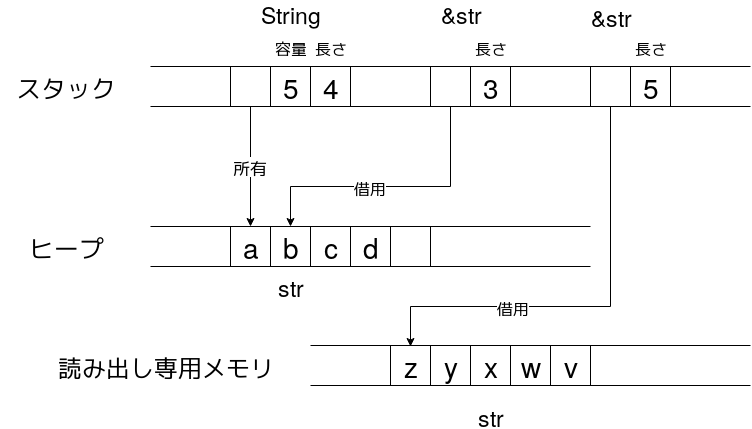
\includegraphics[keepaspectratio,height=4cm]{./image201903/rustlang-str-string.png}
  \label{fig:str-string}
  \caption{RustにおけるStringとstrの違い}
 \end{center}
\end{figure}

\begin{commandline}
fn main() {
    let a = "abcd".to_string(); // String::from("abcd"); でも可
    let b = &a[1..];
    let c = "zyxwv";

    let mut a = "abcd".to_string();
    //  ^^^  aをmutableな変数として宣言
    a.push_str("efg");  // OK

    let mut c = "zyxwv";

    // エラー!: no method named `push_str` found for type `&str` in the current scope
    c.push_str("ut");  // strには追加できないのでpush_strメソッドはない
}
\end{commandline}

\subsubsection{関数定義}

では、関数を定義してみましょう。
Rustでの関数定義は、\texttt{fn}キーワードと`\texttt{->}'トークンを使います。
まずは、単純に足し算を行う関数\texttt{add}を定義してみます。

\begin{commandline}
fn add(a: i32, b: i32) -> i32 {
    return a + b;
}

fn main() {
    println!("{}", add(1, 2));
}
\end{commandline}

これを\texttt{cargo}で実行すると、
(驚くような事は一切ないですが)以下のような結果になります。

\begin{commandline}
% cargo run
Compiling function v0.1.0 (/path/to/examples/function)
Finished dev [unoptimized + debuginfo] target(s) in 0.20s
Running `target/debug/function`
3
\end{commandline}

なお、ここでは\texttt{return}を使いましたが、
Rustではセミコロンを抜かすと値を作るため、
セミコロンを抜かして書いた以下のような\texttt{add}関数も
上記で定義した関数と同じ動作をします(セミコロンを書くとエラーになります)。

\begin{commandline}
fn add(a: i32, b: i32) -> i32 {
    a + b
}
\end{commandline}

\subsubsection{所有権}

さて、ここから一気にRustっぽい話になります。
Rustでは、メモリの安全性が考えられていると書きましたが、
そのために所有権(英語ではownership)という概念を使っています。
C++でもある概念ですが、たとえば以下のようなプログラムがあったとします。

\begin{commandline}
fn main() {
    let i0 = 1;
    let i1 = i0;
    let i2 = i0;

    let s0: String = "hoge".to_string();
    let s1 = s0;
    let s2 = s0;
}
\end{commandline}

さて、どうなると思うでしょうか?
正解は、以下のように\texttt{s2}に\texttt{s0}を代入しているところでエラーになります。

\begin{commandline}
error[E0382]: use of moved value: `s0`
 --> ownership/src/main.rs:8:15
  |
6 |     let s0: String = "hoge".to_string();
  |         -- move occurs because `s0` has type `std::string::String`, which does not implement the `Copy` trait
7 |     let s1 = s0;
  |              -- value moved here
8 |     let s2 = s0;
  |              ^^ value used here after move
\end{commandline}

Rustでは、代入、関数の引数、関数の戻り値などで値の所有権が移動するため、
一度所有権を移譲してしまったら、移譲元の変数はその後アクセスできなくなります(コンパイル時に怒られる)。
ところが、上記のコードでは整数の方はエラーになりません。
これは何故かというと、整数など一部の型(サイズが固定で小さいものが主?)は移動せずにコピーになります。
実はエラーメッセージにあるCopy traitというのがミソで、
整数型はこのCopy traitを実装しているからそういった動作になっています。
traitについては後述します。

関数の引数でも所有権は移動するので、以下のようなコードもアウトです。

\begin{commandline}
fn consume(_s: String) {}

fn main() {
    let h: String = "Hello World".to_string();
    consume(h);
    let hh = h;
}
\end{commandline}

ビルドすると、関数\texttt{consume}コール時に\texttt{h}が移動してしまっているため
以下のようなエラーになります。

\begin{commandline}
12 |     let h: String = "Hello World".to_string();
   |         - move occurs because `h` has type `std::string::String`, which does not implement the `Copy` trait
13 |     consume(h);
   |             - value moved here
14 |     let hh = h;
   |              ^ value used here after move
\end{commandline}

逆に、関数の戻り値でも所有権を移動できるので、以下のようなコードが書けたりします。

\begin{commandline}
fn generate(i: i32) -> Vec<i32> {
    let mut v = Vec::new();
    v.push(i);
    return v;
}

fn main() {
    let v1 = generate(10);
    let mut v2 = generate(100);
    v2.push(101);
    println!("v1: {:?}", v1); // v1: [10]
    println!("v2: {:?}", v2); // v2: [100, 101]
}
\end{commandline}

\subsubsection{参照と借用}

関数呼び出しなどでは、所有権を渡さずに値を使いたい場合が多々あるかと思いますが、
その場合には参照を使います。
なお、Rustでは借用とも言います。
記法としては、C++と同じく\texttt{\&}を使うのですが、
C++とは、
\begin{itemize}
 \item 借用する側(参照される側)に`\texttt{\&}'を付ける
 \item 関数の呼び出し元と呼び出し先両方に`\texttt{\&}'が必要
\end{itemize}
といった点で異なる感じになります。
先程、所有権の移動でエラーになった関数呼び出しのコードを
参照をつかってエラーにならないように書き換えたものが以下になります。

\begin{commandline}
fn consume(_s: &String) {}

fn main() {
    let s0: String = "hoge".to_string();
    let s1 = &s0;
    let s2 = &s0;

    let h: String = "Hello World".to_string();
    consume(&h);
    let hh = h;
}
\end{commandline}

このコードであれば、関数\texttt{consume}をコールしても、
\texttt{h}の所有権はうつっていないため、その後\texttt{hh}に所有権を移譲することができます。
参照の解決には、以下のように\texttt{*}を使います。

\begin{commandline}
fn main() {
    let i0 = 5;
    let i1 = &i0;

    println!("i0: {}, i1: {}", i0, *i1);
}
\end{commandline}

が、関数で使う場合だったり、色々な場面で省略できたりするみたいです。

\begin{commandline}
fn catlength(a: &String, b: &String) -> usize {
    return a.len() + b.len();
}

fn main() {
    let s0 = "hoge".to_string();
    let s1 = "fuga".to_string();
    println!("{}", catlength(&s0, &s1));
}
\end{commandline}

\subsubsection{ライフタイム}

Rustには、GCはなくてC言語のように変数スコープがあり、
スコープを外れた変数は随時消えていきます。
例としては、以下のようなコードを書くと、
ドロップされた後に値を使おうとしているためコンパイル時の怒られます。

\begin{commandline}
fn main() {
    {
        let a = 0;
    }  // ここでドロップ
    println!("{}", a);
}
\end{commandline}

実行すると以下のように怒られます。

\begin{commandline}
error[E0425]: cannot find value `a` in this scope
--> lifetime/src/main.rs:5:20
  |
5 |     println!("{}", a);
  |                    ^ not found in this scope
\end{commandline}

参照している場合とて怒られます。
例として、以下のようなコードを書きます。

\begin{commandline}
fn main() {
    let r;
    {
        let b = 0;
        r = &b;
    }
    println!("{}", r);
}
\end{commandline}

コンパイル時に怒られます。

\begin{commandline}
error[E0597]: `b` does not live long enough
--> lifetime/src/main.rs:11:9
   |
11 |         r = &b;
   |         ^^^^^^ borrowed value does not live long enough
12 |     }
   |     - `b` dropped here while still borrowed
13 |     println!("{}", r);
   |                    - borrow later used here
\end{commandline}

でも、実はこの\textbf{「コンパイル時の怒られる」}というのがミソなのです。
C/C++でよくやる解放済みのメモリアクセスとかが
コンパイル時にみつかるのです。素敵!!
とはいえ、ややこしいのが関数です。以下がエラーになります。

\begin{commandline}
fn longest(x: &str, y: &str) -> &str {
    if x.len() > y.len() {
        x
    } else {
        y
    }
}
\end{commandline}

こんな感じで怒られます。

\begin{commandline}
error[E0106]: missing lifetime specifier
--> lifetime/src/main.rs:1:33
  |
1 | fn longest(x: &str, y: &str) -> &str {
  |                                 ^ expected lifetime parameter
  |
= help: this function's return type contains a borrowed value, but the signature does not say whether it is \
borrowed from `x` or `y`
\end{commandline}

このコードの問題はなにかというと、
実行するまで\texttt{x}と\texttt{y}(どちらも参照)のどちらを返すかわからないので、
戻り値のライフタイムがどうなるかわからないので、
その後の処理がチェックできないという事で怒られています。
ではどうするかというと、コンパイラが言っている通りlifetime parameterを追加します。
具体的には、生存期間\texttt{'a}という表現を用いて以下のように書きます。

\begin{commandline}
fn longest<'a>(x: &'a str, y: &'a str) -> &'a str {
    if x.len() > y.len() {
        x
    } else {
        y
    }
}
\end{commandline}

これによって、この関数\texttt{longest}の戻り値は、
\texttt{x}か\texttt{y}の短い方のライフタイム以上のライフタイムを持つという記載になり、
コンパイラはこれによって値の借用のチェックを行ないます。

\subsubsection{構造体}

Rustにはclassがなく、構造体\texttt{struct}を使います。
定義はC言語の構造体と同じような(型は後置になります)感じですが、
宣言する場合は各要素の名前を逐一書く必要があります。
ただし、要素名と同名の変数で初期化するときのみ省略可能です。
あとは、他の変数から値をコピーして一部だけ値を入れるといった記法もあります。

\begin{commandline}
struct Point {
    x: f64,
    y: f64,
}

fn main() {
    let _p0 = Point { x: 1.0, y: 1.0 };

    let x = 0.0;
    let y = 0.0;
    let _p1 = Point { x, y }; // 変数名とメンバー名が一緒
}
\end{commandline}

なお、構造体ですが、メソッドを生やすことができます。
その際、\texttt{impl}キーワードを用いて、構造体の定義から離れた場所に書きます。
各関数の最初の引数は特別な引数である\texttt{self}への参照である必要があります。
メンバーの値を書き換えたい場合は\texttt{mut}を付けます。

\begin{commandline}
struct Point {
    x: f64,
    y: f64,
}

impl Point {
    fn abs(&self) -> f64 {
        (self.x * self.x + self.y * self.y).sqrt()
    }
}

fn main() {
    let p0 = Point { x: 1.0, y: 1.0 };
    println!("{}", p0.abs()); // => 1.4142135623730951
}
\end{commandline}

\subsubsection{ジェネリック}

C++のテンプレートやJavaのジェネリクスのように、
Rustでも型だけ異なるような関数や構造体を一般的な形で記述することができます。

\begin{commandline}
struct GenPoint<T> {
    x: T,
    y: T,
}

fn main() {
    let _p1 = GenPoint::<i32> { x: 1, y: 1 };
    let _p2 = GenPoint { x: 1, y: 1 };
    let _p3 = GenPoint { x: 1.5, y: 2.0 };
}
\end{commandline}

\subsubsection{trait}

JavaやGoのインターフェース的なものとして、Rustにはトレイト(trait)というものがあります。
さきほど出てきたCopy traitもこれになります。
トレイトは\texttt{trait}キーワードで定義しますが、
たとえばダックタイピングなtraitを書くと以下のようになります。

\begin{commandline}
// Duckは……
trait Duck {
    fn walk(&self);   // walkして
    fn quack(&self);  // quackするもの!!
}
\end{commandline}

この状態で、このDuck traitを実装する構造体を\texttt{impl}キーワードで以下のように作成します。

\begin{commandline}
struct RealDuck {}

impl Duck for RealDuck {
    fn walk(&self) {
        println!("duck walking");
    }

    fn quack(&self) {
        println!("quack")
    }
}

struct Dog {}

impl Duck for Dog {
    fn walk(&self) {
        println!("dog walking");
    }

    fn quack(&self) {
        println!("bow")
    }
}
\end{commandline}

そうすると、以下のように\texttt{Duck}型を引数とする関数\verb|test_duck()|に
\texttt{RealDuck}と\texttt{Dog}のどちらも渡すことができるようになります。

\begin{commandline}
fn test_duck(duck: &Duck) {
    duck.walk();
    duck.quack();
}

fn main() {
    let duck = RealDuck {};
    let dog = Dog {};

    test_duck(&duck);
    test_duck(&dog);
}
\end{commandline}

なお、引数に複数のtraitを実装した型を要求することができます。
たとえば、
\begin{commandline}
fn notify(item: impl Summary + Display) {
\end{commandline}
は2つのtrait、\verb|Summary|と\verb|Display|を同時に実装した型を引数\texttt{item}に要求します。
これだと読みづらい感じもするので、以下の書き型もできます。
\begin{commandline}
fn notify<T: Summary + Display>(item: T) {
\end{commandline}
また、引数が一杯になってきたら上記でも辛いので、以下のような\texttt{where}をつかって記法もあります。
\begin{commandline}
fn some_function<T, U>(t: T, u: U) -> i32
    where T: Display + Clone,
          U: Clone + Debug
{
\end{commandline}

\subsubsection{enum}

さて、enumです。個人的にはかなり気にいってますが、
Rustのenumは、ちょっとおかしなくらいに色々とできます。
もちろん、C言語のような以下のようなenumは作れます。

\begin{commandline}
enum Fruits {
    Apple,
    Banana,
    Orange,
    Peach,
}

fn main() {
    let _hoge = Fruits::Apple;
}
\end{commandline}

が、Rustのenumは、各値の中にさらに値を持たせることができます。
しかも、型や値の個数はバラバラで構いません。
たとえば、以下のようなenumを定義できます。
なお、ここで出てきている\texttt{(u8, u8, u8, u8)}というのは
8-bit符号無し整数を4つ持つタプル型です。

\begin{commandline}
enum IpAddr {
    V4((u8, u8, u8, u8)),
    V6(String),
}
\end{commandline}

このように定義してあげると、実際の値を作る際、
以下のように値を入れてenumの値を作ることができます。

\begin{commandline}
fn main() {
    let v4_addr = IpAddr::V4((127, 0, 0, 1));
    let v6_addr = IpAddr::V6("::1".into());
}
\end{commandline}

このようにして作った値は、\texttt{match}を使って値を取り出せます。
C言語の\texttt{switch}文的な感じで使えます。
以下のコードはenum値全てのケースを記述していますが、
\texttt{default}的な処理は``\verb|_ => { /* 処理 */ }|''として書けます。

\begin{commandline}
fn extract_addr(addr: &IpAddr) {
    match addr {
        IpAddr::V4(a) => {
            println!("{}.{}.{}.{}", a.0, a.1, a.2, a.3);
        }
        IpAddr::V6(a) => {
            println!("{}", a);
        }
    }
}

fn main() {
    extract_addr(&v4_addr); // => 127.0.0.1
    extract_addr(&v6_addr); // => ::1
}
\end{commandline}

\subsubsection{\texttt{Option<T>}と\texttt{Result<T,E>}}

Rustには例外もnullptrもありませんが、その代わりにジェネリックなenumである
\texttt{Option<T>}と\texttt{Result<T,E>}を使ってエラー等を処理します。
それぞれの機能をざっくり説明すると、
\begin{itemize}
  \item \verb|Option<T>|
	\begin{itemize}
	 \item 値がない可能性がある事を示す (nullptrの代わり)
	\end{itemize}
 \item \verb|Result<T,E>|
       \begin{itemize}
	\item 失敗する可能性がある事を示す (例外の代わり)
       \end{itemize}
\end{itemize}
といった感じでしょうか。
それぞれの定義は以下のようにされています。

\begin{commandline}
pub enum Option<T> {
    None,
    Some(T),
}

pub enum Result<T, E> {
    Ok(T),
    Err(E),
}
\end{commandline}

例えば、1つ目のコマンドライン引数を受けとり、
それをi32型に変更して表示する関数を書くと次のようになります。
まず引数が一つも無い場合があるため、引数があれば\texttt{Some()}の中身に引数が、
なければ\texttt{None}が取り出されます。
その後、\texttt{Some()}の中身を取り出しますが、
i32型としてパースできない場合があるため、成功したか失敗したかを
\texttt{Ok()}か\texttt{Err()}かで判定しています。

\begin{commandline}
use std::env;

fn main() {
    let i = match env::args().nth(1) {
        None => {
            panic!("no arguments");
        }
        Some(arg) => match arg.parse::<i32>() {
            Ok(fig) => fig,
            Err(e) => {
                panic!("error: {}", e);
            }
        },
    };

    println!("i: {}", i);
}
\end{commandline}

実際には、上記の処理をもうちょっと綺麗に書けるように
\texttt{?}演算子や\texttt{expect()}メソッドなどが定義されています。
が、ここでは詳細は省きます。

\subsubsection{crate}

Rustのプログラムは、クレート(crate)と呼ばれる単位の組み合わせで構成されます。
今回は、詳細については割愛して、
crates.io\footnote{\url{https://crates.io/}}にて公開されている
クレートの使い方について簡単に紹介します。
といっても、実はとても簡単で、cargoの設定ファイルのCargo.tomlに
crates.ioで使いたいクレートのページに掲載されている式を貼り付けるだけです。

今回はオプション解析のクレートであるclap\footnote{\url{https://clap.rs/}}を使ってみましょう。
サイトにある式を、Cargo.tomlの[dependencies]の項目に追記してあげればOKです。

\begin{commandline}
[dependencies]
clap = "2.32.0"
\end{commandline}

では、これをつかって、簡単なプログラムを作ってみます。
とりあえず、\verb|-n|オプションだけあるような
似非echoコマンドを以下のように書いてみました。

\begin{commandline}
use clap::{App, Arg};

fn main() {
    let m = App::new("echo")  // コマンド名
        .arg(Arg::with_name("STRING").multiple(true))  // 複数の引数
        .arg( // '-n' を定義
            Arg::with_name("n")
                .short("n")
                .help("do not output the trailing newline"),
        )
        .get_matches();  // 実行

    let out = match m.values_of("STRING") {
        //         ↓地味にイテレータを使用
        Some(v) => v.collect::<Vec<&str>>().join(" "),
        None => "".into(),
    };

    print!("{}", out);

    if !m.is_present("n") {
        println!("");  // '-n'オプションがなければ改行
    }
}
\end{commandline}

Rust 2018 Editionと呼ばれる2018年の年末にリリースされたバージョン以降では、
これまで必要だった\verb|extern crate clap;|という記述が不要になっています。

ということで、ここまでかなり高速にRustの構文等の紹介をしてきましたが、
まったくもって極一部ですので、興味があればThe Bookを読んでもらえればと思います。

\subsection{Debianパッケージにしてみる}

ここでようやくDebianな話題ですが、ひとまずここでは先程作成したclapで作った似非echoコマンドを
debianパッケージにしてみるということをやります。

Rustの単一バイナリのdebianパッケージ化について、
一番簡単なのは\texttt{cargo}のサブコマンド用の
\texttt{cargo-deb}%
\footnote{\url{https://github.com/mmstick/cargo-deb}}%
を用いる方法があるようです。
あるようなんですが……残念ながらこのツール、
とても公式に入れられないようなdebしか吐かないようです。
ドキュメントもないし云々。
まぁ、/usr/binにえいやと入れたいならアリかもですが。

で、さすがにそれだとアレなので、もうちょっとちゃんとしたdebを作るべく、
Debian Rust packaging teamのWiki%
\footnote{\url{https://wiki.debian.org/Teams/RustPackaging}}%
に、それなりにしたがってみようかと思います。
どうやら、crates.ioにあるcrateについては、
debcargo\footnote{\url{https://salsa.debian.org/rust-team/debcargo}}%
というツールを使うと良い感じに処理してくれるようです。
が、今回はcrate.ioにはアップされていないもので作りたいという話なんですが、
debcargoは対応していなさそうです。
そのため、debcargoが使っているdh-cargoをつかって地道に対応してみることにしました。

まずは、dh\_makeを実行してdebianディレクトリを作り、
できあがったdebian/rulesのbuildルールのdhにオプション\verb|--byildsystem cargo|を追加することと、
debian/controlのBuild-Dependsにdh-cargoとlibrust-clap-devを追加してみました。
ひとまずここでビルドしてみます。

\begin{commandline}
% debuild-pbuilder
-> Attempting to satisfy build-dependencies
-> Creating pbuilder-satisfydepends-dummy package
Package: pbuilder-satisfydepends-dummy
Version: 0.invalid.0

... (snip) ...

dh_autoreconf -O--buildsystem=cargo
dh_auto_configure -O--buildsystem=cargo
cp: './debian/cargo-checksum.json' を stat できません: そのようなファイルやディレクトリはありません
\end{commandline}

なにかファイルがないと言われてしまいました。
Wikiを見ると、どうやらupstreamのcrateのチェックサムを含めたファイルを
用意してやる必要があるようです。
これは、/usr/share/cargo/registry以下にdebでインストールされた
ライブラリたちを使うためのようなのですが、
あまりWikiを読んでも作り方がわかりませんでした。
どうも、cargo-vendorというツールを利用していそうなのですが……。
とか思っていたのですが、

\begin{commandline}
% apt source ripgrep
% cat rust-ripgrep-0.10.0/debian/cargo-checksum.json
{"package":"Could not get crate checksum","files":{}}
\end{commandline}

と、公式のripgrepのdebのソースをみると、このファイルが哀しいことになっていました。
それでもちゃんとビルドは通るようです。
ためしに、debian/cargo-checksum.jsonをtouchで空ファイルとして作ってみたら、
普通にビルドが進んでしまいました。いったんわすれます……。

ところが、まだコケます。

\begin{commandline}
debian cargo wrapper: running subprocess (['env', 'RUST_BACKTRACE=1', '/usr/bin/cargo', '-Zavoid-dev-deps', \
'build', '--verbose', '--verbose', '-j4', '--target', 'x86_64-unknown-linux-gnu'],) {}
error: failed to select a version for the requirement `textwrap = "= 0.10.0"`
candidate versions found which didn't match: 0.11.0
location searched: directory source `/path/to/clap-test/debian/cargo_registry` (which is replacing registry \
`https://github.com/rust-lang/crates.io-index`)
required by package `clap v2.32.0`
\end{commandline}

clapが依存しているtextwrapのバージョンが0.10.0だけど、手元にあるのは0.11.0だと。
たしかに、textwrapのdebのバージョンは0.11.0でした。
が、そうなるとおなじくclapを使っているripgrepのビルドが通っているのが解せません。
と調べていくと、GitHubのリポジトリ\footnote{\url{https://github.com/BurntSushi/ripgrep}}に
置いてあるバージョンとripgrepのdebのorigソースを見比べると、
Cargo.tomlが若干異なり、Cargo.lockが編集されていることがわかりました。
そして、消されたCargo.lockの中には、textwrapの0.10.0のチェックサムが記載されています。
そもそも、Cargo.tomlはで開発者がざっくりとした依存を書くファイルで、
Cargo.lockは、cargoが実情に基づいて自動で生成し、
\verb|cargo update|などすることによってバージョンが更新されるものです。

で、確認していくと、どうやら/usr/share/cargo/registry以下にあるtextwrapの
Cargo.tomlのtextwrapの依存がcrates.io登録時に以下のように書きかわっていることがわかりました。

\begin{commandline}
% grep -A 1 dependencies.textwrap debian/cargo_registry/clap-2.32.0/Cargo.toml
[dependencies.textwrap]
version = ">= 0.10, < 0.12"
\end{commandline}

ちなみに、GitHubのclapのコードには以下としか書いてないです。

\begin{commandline}
[dependencies]
bitflags              = "1.0"
unicode-width         = "0.1.4"
textwrap              = "0.10.0"
\end{commandline}

ということで、変更の基準はまったくわかってませんが(今後の課題とさせていただきます!!)、
今回の似非echoコマンドについては、Cargo.lockを消せば最後までビルドされました。
lintianのエラーも警告も取れてないですが、ひとまず動きますよ!!

\begin{commandline}
% dpkg -I rust-clap-test_0.1.0-1_amd64.deb
new Debian package, version 2.0.
size 258160 bytes: control archive=648 bytes.
360 バイト、   11 行      control
285 バイト、    4 行      md5sums
Package: rust-clap-test
Version: 0.1.0-1
Architecture: amd64
Maintainer: Katsuki Kobayashi <rare@tirasweel.org>
Installed-Size: 770
Depends: libc6 (>= 2.18), libgcc1 (>= 1:4.2)
Section: unknown
Priority: optional
Homepage: <insert the upstream URL, if relevant>
Description: <insert up to 60 chars description>
<insert long description, indented with spaces>

% dpkg -c rust-clap-test_0.1.0-1_amd64.deb
drwxr-xr-x root/root         0 2019-03-23 18:06 ./
drwxr-xr-x root/root         0 2019-03-23 18:06 ./usr/
drwxr-xr-x root/root         0 2019-03-23 18:06 ./usr/bin/
-rwxr-xr-x root/root    776600 2019-03-23 18:06 ./usr/bin/clap-test
drwxr-xr-x root/root         0 2019-03-23 18:06 ./usr/share/
drwxr-xr-x root/root         0 2019-03-23 18:06 ./usr/share/doc/
drwxr-xr-x root/root         0 2019-03-23 18:06 ./usr/share/doc/rust-clap-test/
-rw-r--r-- root/root       197 2019-03-23 18:06 ./usr/share/doc/rust-clap-test/README.Debian
-rw-r--r-- root/root       190 2019-03-23 18:06 ./usr/share/doc/rust-clap-test/changelog.Debian.gz
-rw-r--r-- root/root      1693 2019-03-23 18:06 ./usr/share/doc/rust-clap-test/copyright
\end{commandline}

\subsection{まとめ}

ということで、しりすぼみ感は拭えませんが、
結局Rustなdebを作るには、現状ではcrates.ioに登録してdebcargoをベースにつくる
というのが公式のようでした。
が、もちろんdh-cargoがあるのでcrates.ioに登録しなくてもdebにはできそうです。
cargo自体は、外部クレートにgitリポジトリを指定したりできるので、
debcargoもgitリポジトリに対応できたら良いですが、今回のCargo.toml/Cargo.lockを
crates.ioが編集している兼ね合いもあるので、色々と大変かもしれません。

というか、そもそもlibrust-*パッケージ達の依存関係はあやしいのかもしれません。
つい先日も、ripgrepがビルドできないというバグも報告されていましたし%
\footnote{\url{https://bugs.debian.org/cgi-bin/bugreport.cgi?bug=920958}}。
とは言え、debcargo自体は粛々と開発が進んでいるようで、
これを書いてる直前くらいにも、busterには入らないけど
post-installでtestができるようになったり%
\footnote{\url{https://alioth-lists.debian.net/pipermail/pkg-rust-maintainers/2019-March/005296.html}}%
しているようです。
なんにせよ、Rust自体は良い言語かと思うので、
今後流行っていけば良いなぁと思います。


\clearpage
\newpage

%-------------------------------------------------------------------------------
%\dancersection{Debian Trivia Quiz}{ }
%-------------------------------------------------------------------------------

%ところで、みなさん Debian 関連の話題においついていますか?Debian関連の話
%題はメーリングリストをよんでいると追跡できます。ただよんでいるだけではは
%りあいがないので、理解度のテストをします。特に一人だけでは意味がわからな
%いところもあるかも知れません。みんなで一緒に読んでみましょう。

%今回の出題範囲は\url{debian-devel-announce@lists.debian.org} や \url{debian-devel@lists.debian.org}に投稿された
%内容とDebian Project Newsからです。

%\begin{multicols}{2}
%\end{multicols}

% 索引
%\printindex
\clearpage
\begin{center}
本資料のライセンスについて
\end{center}

本資料はフリー・ソフトウェアです。あなたは、Free Software
Foundation が公表したGNU GENERAL PUBLIC LICENSEの "バージョン2"もしくはそれ以降
が定める条項に従って本プログラムを再頒布または変更することができ
ます。

本プログラムは有用とは思いますが、頒布にあたっては、市場性及び特
定目的適合性についての暗黙の保証を含めて、いかなる保証も行ないま
せん。詳細についてはGNU GENERAL PUBLIC LICENSE をお読みください。

\begin{multicols}{2}
 \begin{fontsize}{6}{6}
 \begin{verbatim}
            GNU GENERAL PUBLIC LICENSE
               Version 2, June 1991

 Copyright (C) 1989, 1991 Free Software Foundation, Inc.
    51 Franklin St, Fifth Floor, Boston, MA  02110-1301  USA
 Everyone is permitted to copy and distribute verbatim copies
 of this license document, but changing it is not allowed.

                Preamble

  The licenses for most software are designed to take away your
freedom to share and change it.  By contrast, the GNU General Public
License is intended to guarantee your freedom to share and change free
software--to make sure the software is free for all its users.  This
General Public License applies to most of the Free Software
Foundation's software and to any other program whose authors commit to
using it.  (Some other Free Software Foundation software is covered by
the GNU Library General Public License instead.)  You can apply it to
your programs, too.

  When we speak of free software, we are referring to freedom, not
price.  Our General Public Licenses are designed to make sure that you
have the freedom to distribute copies of free software (and charge for
this service if you wish), that you receive source code or can get it
if you want it, that you can change the software or use pieces of it
in new free programs; and that you know you can do these things.

  To protect your rights, we need to make restrictions that forbid
anyone to deny you these rights or to ask you to surrender the rights.
These restrictions translate to certain responsibilities for you if you
distribute copies of the software, or if you modify it.

  For example, if you distribute copies of such a program, whether
gratis or for a fee, you must give the recipients all the rights that
you have.  You must make sure that they, too, receive or can get the
source code.  And you must show them these terms so they know their
rights.

  We protect your rights with two steps: (1) copyright the software, and
(2) offer you this license which gives you legal permission to copy,
distribute and/or modify the software.

  Also, for each author's protection and ours, we want to make certain
that everyone understands that there is no warranty for this free
software.  If the software is modified by someone else and passed on, we
want its recipients to know that what they have is not the original, so
that any problems introduced by others will not reflect on the original
authors' reputations.

  Finally, any free program is threatened constantly by software
patents.  We wish to avoid the danger that redistributors of a free
program will individually obtain patent licenses, in effect making the
program proprietary.  To prevent this, we have made it clear that any
patent must be licensed for everyone's free use or not licensed at all.

  The precise terms and conditions for copying, distribution and
modification follow.

            GNU GENERAL PUBLIC LICENSE
   TERMS AND CONDITIONS FOR COPYING, DISTRIBUTION AND MODIFICATION

  0. This License applies to any program or other work which contains
a notice placed by the copyright holder saying it may be distributed
under the terms of this General Public License.  The "Program", below,
refers to any such program or work, and a "work based on the Program"
means either the Program or any derivative work under copyright law:
that is to say, a work containing the Program or a portion of it,
either verbatim or with modifications and/or translated into another
language.  (Hereinafter, translation is included without limitation in
the term "modification".)  Each licensee is addressed as "you".

Activities other than copying, distribution and modification are not
covered by this License; they are outside its scope.  The act of
running the Program is not restricted, and the output from the Program
is covered only if its contents constitute a work based on the
Program (independent of having been made by running the Program).
Whether that is true depends on what the Program does.

  1. You may copy and distribute verbatim copies of the Program's
source code as you receive it, in any medium, provided that you
conspicuously and appropriately publish on each copy an appropriate
copyright notice and disclaimer of warranty; keep intact all the
notices that refer to this License and to the absence of any warranty;
and give any other recipients of the Program a copy of this License
along with the Program.

You may charge a fee for the physical act of transferring a copy, and
you may at your option offer warranty protection in exchange for a fee.

  2. You may modify your copy or copies of the Program or any portion
of it, thus forming a work based on the Program, and copy and
distribute such modifications or work under the terms of Section 1
above, provided that you also meet all of these conditions:

    a) You must cause the modified files to carry prominent notices
    stating that you changed the files and the date of any change.

    b) You must cause any work that you distribute or publish, that in
    whole or in part contains or is derived from the Program or any
    part thereof, to be licensed as a whole at no charge to all third
    parties under the terms of this License.

    c) If the modified program normally reads commands interactively
    when run, you must cause it, when started running for such
    interactive use in the most ordinary way, to print or display an
    announcement including an appropriate copyright notice and a
    notice that there is no warranty (or else, saying that you provide
    a warranty) and that users may redistribute the program under
    these conditions, and telling the user how to view a copy of this
    License.  (Exception: if the Program itself is interactive but
    does not normally print such an announcement, your work based on
    the Program is not required to print an announcement.)

These requirements apply to the modified work as a whole.  If
identifiable sections of that work are not derived from the Program,
and can be reasonably considered independent and separate works in
themselves, then this License, and its terms, do not apply to those
sections when you distribute them as separate works.  But when you
distribute the same sections as part of a whole which is a work based
on the Program, the distribution of the whole must be on the terms of
this License, whose permissions for other licensees extend to the
entire whole, and thus to each and every part regardless of who wrote it.

Thus, it is not the intent of this section to claim rights or contest
your rights to work written entirely by you; rather, the intent is to
exercise the right to control the distribution of derivative or
collective works based on the Program.

In addition, mere aggregation of another work not based on the Program
with the Program (or with a work based on the Program) on a volume of
a storage or distribution medium does not bring the other work under
the scope of this License.

  3. You may copy and distribute the Program (or a work based on it,
under Section 2) in object code or executable form under the terms of
Sections 1 and 2 above provided that you also do one of the following:

    a) Accompany it with the complete corresponding machine-readable
    source code, which must be distributed under the terms of Sections
    1 and 2 above on a medium customarily used for software interchange; or,

    b) Accompany it with a written offer, valid for at least three
    years, to give any third party, for a charge no more than your
    cost of physically performing source distribution, a complete
    machine-readable copy of the corresponding source code, to be
    distributed under the terms of Sections 1 and 2 above on a medium
    customarily used for software interchange; or,

    c) Accompany it with the information you received as to the offer
    to distribute corresponding source code.  (This alternative is
    allowed only for noncommercial distribution and only if you
    received the program in object code or executable form with such
    an offer, in accord with Subsection b above.)

The source code for a work means the preferred form of the work for
making modifications to it.  For an executable work, complete source
code means all the source code for all modules it contains, plus any
associated interface definition files, plus the scripts used to
control compilation and installation of the executable.  However, as a
special exception, the source code distributed need not include
anything that is normally distributed (in either source or binary
form) with the major components (compiler, kernel, and so on) of the
operating system on which the executable runs, unless that component
itself accompanies the executable.

If distribution of executable or object code is made by offering
access to copy from a designated place, then offering equivalent
access to copy the source code from the same place counts as
distribution of the source code, even though third parties are not
compelled to copy the source along with the object code.

  4. You may not copy, modify, sublicense, or distribute the Program
except as expressly provided under this License.  Any attempt
otherwise to copy, modify, sublicense or distribute the Program is
void, and will automatically terminate your rights under this License.
However, parties who have received copies, or rights, from you under
this License will not have their licenses terminated so long as such
parties remain in full compliance.

  5. You are not required to accept this License, since you have not
signed it.  However, nothing else grants you permission to modify or
distribute the Program or its derivative works.  These actions are
prohibited by law if you do not accept this License.  Therefore, by
modifying or distributing the Program (or any work based on the
Program), you indicate your acceptance of this License to do so, and
all its terms and conditions for copying, distributing or modifying
the Program or works based on it.

  6. Each time you redistribute the Program (or any work based on the
Program), the recipient automatically receives a license from the
original licensor to copy, distribute or modify the Program subject to
these terms and conditions.  You may not impose any further
restrictions on the recipients' exercise of the rights granted herein.
You are not responsible for enforcing compliance by third parties to
this License.

  7. If, as a consequence of a court judgment or allegation of patent
infringement or for any other reason (not limited to patent issues),
conditions are imposed on you (whether by court order, agreement or
otherwise) that contradict the conditions of this License, they do not
excuse you from the conditions of this License.  If you cannot
distribute so as to satisfy simultaneously your obligations under this
License and any other pertinent obligations, then as a consequence you
may not distribute the Program at all.  For example, if a patent
license would not permit royalty-free redistribution of the Program by
all those who receive copies directly or indirectly through you, then
the only way you could satisfy both it and this License would be to
refrain entirely from distribution of the Program.

If any portion of this section is held invalid or unenforceable under
any particular circumstance, the balance of the section is intended to
apply and the section as a whole is intended to apply in other
circumstances.

It is not the purpose of this section to induce you to infringe any
patents or other property right claims or to contest validity of any
such claims; this section has the sole purpose of protecting the
integrity of the free software distribution system, which is
implemented by public license practices.  Many people have made
generous contributions to the wide range of software distributed
through that system in reliance on consistent application of that
system; it is up to the author/donor to decide if he or she is willing
to distribute software through any other system and a licensee cannot
impose that choice.

This section is intended to make thoroughly clear what is believed to
be a consequence of the rest of this License.

  8. If the distribution and/or use of the Program is restricted in
certain countries either by patents or by copyrighted interfaces, the
original copyright holder who places the Program under this License
may add an explicit geographical distribution limitation excluding
those countries, so that distribution is permitted only in or among
countries not thus excluded.  In such case, this License incorporates
the limitation as if written in the body of this License.

  9. The Free Software Foundation may publish revised and/or new versions
of the General Public License from time to time.  Such new versions will
be similar in spirit to the present version, but may differ in detail to
address new problems or concerns.

Each version is given a distinguishing version number.  If the Program
specifies a version number of this License which applies to it and "any
later version", you have the option of following the terms and conditions
either of that version or of any later version published by the Free
Software Foundation.  If the Program does not specify a version number of
this License, you may choose any version ever published by the Free Software
Foundation.

  10. If you wish to incorporate parts of the Program into other free
programs whose distribution conditions are different, write to the author
to ask for permission.  For software which is copyrighted by the Free
Software Foundation, write to the Free Software Foundation; we sometimes
make exceptions for this.  Our decision will be guided by the two goals
of preserving the free status of all derivatives of our free software and
of promoting the sharing and reuse of software generally.

                NO WARRANTY

  11. BECAUSE THE PROGRAM IS LICENSED FREE OF CHARGE, THERE IS NO WARRANTY
FOR THE PROGRAM, TO THE EXTENT PERMITTED BY APPLICABLE LAW.  EXCEPT WHEN
OTHERWISE STATED IN WRITING THE COPYRIGHT HOLDERS AND/OR OTHER PARTIES
PROVIDE THE PROGRAM "AS IS" WITHOUT WARRANTY OF ANY KIND, EITHER EXPRESSED
OR IMPLIED, INCLUDING, BUT NOT LIMITED TO, THE IMPLIED WARRANTIES OF
MERCHANTABILITY AND FITNESS FOR A PARTICULAR PURPOSE.  THE ENTIRE RISK AS
TO THE QUALITY AND PERFORMANCE OF THE PROGRAM IS WITH YOU.  SHOULD THE
PROGRAM PROVE DEFECTIVE, YOU ASSUME THE COST OF ALL NECESSARY SERVICING,
REPAIR OR CORRECTION.

  12. IN NO EVENT UNLESS REQUIRED BY APPLICABLE LAW OR AGREED TO IN WRITING
WILL ANY COPYRIGHT HOLDER, OR ANY OTHER PARTY WHO MAY MODIFY AND/OR
REDISTRIBUTE THE PROGRAM AS PERMITTED ABOVE, BE LIABLE TO YOU FOR DAMAGES,
INCLUDING ANY GENERAL, SPECIAL, INCIDENTAL OR CONSEQUENTIAL DAMAGES ARISING
OUT OF THE USE OR INABILITY TO USE THE PROGRAM (INCLUDING BUT NOT LIMITED
TO LOSS OF DATA OR DATA BEING RENDERED INACCURATE OR LOSSES SUSTAINED BY
YOU OR THIRD PARTIES OR A FAILURE OF THE PROGRAM TO OPERATE WITH ANY OTHER
PROGRAMS), EVEN IF SUCH HOLDER OR OTHER PARTY HAS BEEN ADVISED OF THE
POSSIBILITY OF SUCH DAMAGES.

             END OF TERMS AND CONDITIONS

        How to Apply These Terms to Your New Programs

  If you develop a new program, and you want it to be of the greatest
possible use to the public, the best way to achieve this is to make it
free software which everyone can redistribute and change under these terms.

  To do so, attach the following notices to the program.  It is safest
to attach them to the start of each source file to most effectively
convey the exclusion of warranty; and each file should have at least
the "copyright" line and a pointer to where the full notice is found.

    <one line to give the program's name and a brief idea of what it does.>
    Copyright (C) <year>  <name of author>

    This program is free software; you can redistribute it and/or modify
    it under the terms of the GNU General Public License as published by
    the Free Software Foundation; either version 2 of the License, or
    (at your option) any later version.

    This program is distributed in the hope that it will be useful,
    but WITHOUT ANY WARRANTY; without even the implied warranty of
    MERCHANTABILITY or FITNESS FOR A PARTICULAR PURPOSE.  See the
    GNU General Public License for more details.

    You should have received a copy of the GNU General Public License
    along with this program; if not, write to the Free Software
    Foundation, Inc., 51 Franklin St, Fifth Floor, Boston, MA  02110-1301 USA


Also add information on how to contact you by electronic and paper mail.

If the program is interactive, make it output a short notice like this
when it starts in an interactive mode:

    Gnomovision version 69, Copyright (C) year  name of author
    Gnomovision comes with ABSOLUTELY NO WARRANTY; for details type `show w'.
    This is free software, and you are welcome to redistribute it
    under certain conditions; type `show c' for details.

The hypothetical commands `show w' and `show c' should show the appropriate
parts of the General Public License.  Of course, the commands you use may
be called something other than `show w' and `show c'; they could even be
mouse-clicks or menu items--whatever suits your program.

You should also get your employer (if you work as a programmer) or your
school, if any, to sign a "copyright disclaimer" for the program, if
necessary.  Here is a sample; alter the names:

  Yoyodyne, Inc., hereby disclaims all copyright interest in the program
  `Gnomovision' (which makes passes at compilers) written by James Hacker.

  <signature of Ty Coon>, 1 April 1989
  Ty Coon, President of Vice

This General Public License does not permit incorporating your program into
proprietary programs.  If your program is a subroutine library, you may
consider it more useful to permit linking proprietary applications with the
library.  If this is what you want to do, use the GNU Library General
Public License instead of this License.
 \end{verbatim}
 \end{fontsize}
\end{multicols}

\begin{center}
ソースコードについて
\end{center}

このプログラムは \TeX で記述されたものです。ソースコードは
\begin{center}
  \url{https://salsa.debian.org/tokyodebian-team/monthly-report.git}
\end{center}
から取得できます。

\begin{center}
Debian オープンユーズロゴ ライセンス
\end{center}

\begin{multicols}{2}
 \begin{fontsize}{6}{6}
 \begin{verbatim}

Copyright (c) 1999 Software in the Public Interest
Permission is hereby granted, free of charge, to any person
obtaining a copy of this software and associated documentation
files (the "Software"), to deal in the Software without restriction,
including without limitation the rights to use, copy, modify, merge,
publish, distribute, sublicense, and/or sell copies of the Software,
and to permit persons to whom the Software is furnished to do so,
subject to the following conditions:

The above copyright notice and this permission notice shall be
included in all copies or substantial portions of the Software.

THE SOFTWARE IS PROVIDED "AS IS", WITHOUT WARRANTY OF ANY
KIND, EXPRESS OR IMPLIED, INCLUDING BUT NOT LIMITED TO THE
WARRANTIES OF MERCHANTABILITY, FITNESS FOR A PARTICULAR PURPOSE AND
NONINFRINGEMENT. IN NO EVENT SHALL THE AUTHORS OR COPYRIGHT HOLDERS
BE LIABLE FOR ANY CLAIM, DAMAGES OR OTHER LIABILITY, WHETHER IN
AN ACTION OF CONTRACT, TORT OR OTHERWISE, ARISING FROM, OUT OF OR
IN CONNECTION WITH THE SOFTWARE OR THE USE OR OTHER DEALINGS IN
THE SOFTWARE.
 \end{verbatim}
 \end{fontsize}
\end{multicols}

% 問題と回答が同じみひらきにならないようにする
%\cleartoevenpage
%-------------------------------------------------------------------------------
%\dancersection{Debian Trivia Quiz 問題回答}{ }
%-------------------------------------------------------------------------------
%\\
%{\small
% Debian Trivia Quiz の問題回答です。 あなたは何問わかりましたか? \\
 %回答はdebianmeetingresume2016-natsu.jqzというファイルに生成されるので、
 %それを手動でコピペして使う。
 % ここからコピペ
 % FIXME 問題が全部はいったらコピペすること
\pagestyle{empty}
\cleartoevenpage
 
\pagestyle{empty}
\cleartoevenpage

\newpage
{
\large
\begin{itembox}{\bf 『あんどきゅめんてっど でびあん』について}
% FIXME: 対象を修正すること。
本書は、東京および関西周辺で毎月行なわれている『東京エリア Debian 勉強会』(2018年12月-2019年5月,2019年7月)および
『関西 Debian 勉強会』(2018年12月-2019年5月)で使用された資料・小ネタ・必殺技などを一冊にまとめたものです。
内容は無保証、つっこみなどがあれば勉強会にて。
\end{itembox}
}

\vspace*{13cm}
{\color{dancerlightblue}\rule{\hsize}{1mm}}
\vspace{2mm}

\includegraphics[width=2cm]{image200502/openlogo-nd.eps}
\noindent \Large \bf あんどきゅめんてっど でびあん 2019年夏号\\
\noindent \normalfont 2019年8月12日 \hspace{5mm}  初版第1刷発行\\
\noindent \normalfont 東京エリア Debian 勉強会/関西エリア Debian 勉強会 (編集・印刷・発行)\\
{\color{dancerdarkblue}\rule{\hsize}{1mm}}

\end{document}
